\chapter{Разработка модели сухого электронно-лучевого травления резиста}

В данной главе описывается процесс разработки модели сухого электронно-лучевого травления резиста. Большая часть главы посвящена описанию моделей отдельных процессов, протекающих при СЭЛТР. Модель рассеяния электронного пучка в веществе, модель диффузии мономера из слоя ПММА и модель нагрева слоя ПММА при экспонировании были использованы в том виде, в котором они приводятся в литературе, с небольшими изменениями. В свою очередь, модель электронно-стимулированных разрывов молекул ПММА, модель электронно-стимулированной термической деполимеризации ПММА и модель процессов растекания слоя ПММА в процессе СЭЛТР были разработаны впервые в рамках данной работы. Объединение моделей вышеописанных процессов позволило получить модель всего процесса СЭЛТР и определить механизм формирования рельефа, получаемого методом СЭЛТР. Также в этой главе описаны экспериментальные методы, применявшиеся при формировании структур методом СЭЛТР и получении их профилей, использовавшихся для верификации разработанной модели процесса СЭЛТР.

\section{Модель рассеяния электронного пучка в системе ПММА/Si}

Для моделирования рассеяния электронного пучка в системе ПММА/Si в данной работе был реализован алгоритм на основе метода Монте-Карло.
Для описания процессов упругого рассеяния использовались моттовские сечения упругого рассеяния, рассчитанные с использованием свободно распространяемой программы ``ELSEPA''~\cite{ELSEPA}.
Для описания процессов неупругого рассеяния электронного пучка в ПММА была использована модель, учитывающая электрон-электронное, электрон-фононное и электрон-поляронное рассеяние~\cite{Ciappa_2010}. Для описания процессов неупругого рассеяния в кремнии использовался подход, в котором функция потерь энергии вещества представляется в виде суммы функций потерь энергии осцилляторов Друде с квадратичным законом дисперсии~\cite{Valentin2012_Si}.
Данный алгоритм позволил промоделировать акты электрон-электронного рассеяния в \linebreak ПММА, распределение которых в дальнейшем использовалось для моделирования распределения электронно-стимулированных разрывов молекул ПММА.

\section{Модель электронно-стимулированных разрывов молекул ПММА}
Для моделирования электронно-стимулированных разрывов молекул \linebreak ПММА был разработан подход, основанный на предположении, что разрыв молекулы происходит при электрон-электронном рассеянии с вероятностью $\ps$.
В этом случае экспериментально наблюдаемое увеличение радиационно-химического выхода разрывов $\Gs$ с ростом температуры может быть описано за счет увеличения $\ps$.
Для нахождения зависимости $\ps$ от температуры было проведено моделирование эксперимента по определению $\Gs$ на основе значений среднечисловой молекулярной массы резиста до и после экспонирования.
Параметры эксперимента были взяты из работы~\cite{Harris_G_value}: толщина слоя ПММА -- 500~нм, энергия электронного пучка -- 10 кэВ, доза экспонирования -- 100 мкКл/см$\pp$. Начальные значения среднечисловой и средневесовой молекулярной массы ПММА составляли 563000 и 2260000 соответственно.

Для моделирования среднечисловой молекулярной массы проэкспонированного ПММА была специально разработана модель слоя ПММА, предоставляющая подробную информацию о молекулярно-массовом распределении \linebreak ПММА.
Изначально на основе модели идеальной цепи~\cite{Han_2003} были промоделированы отдельные молекулы, длины которых согласовывались с начальным молекулярно-массовым распределением ПММА~\cite{Harris_G_value}.
Далее для каждой молекулы случайным образом выбиралось положение внутри области размерами 100$\times$100$\times$500 нм$\ppp$ с учетом периодических граничных условия.
Область заполнялась молекулами до тех пор, пока не была достигнута необходимая плотность (1.19 г/см$\ppp$) (рисунок~\ref{fig:Harris_chains}).

\begin{figure}[t!]
	\begin{minipage}{0.48\textwidth}
		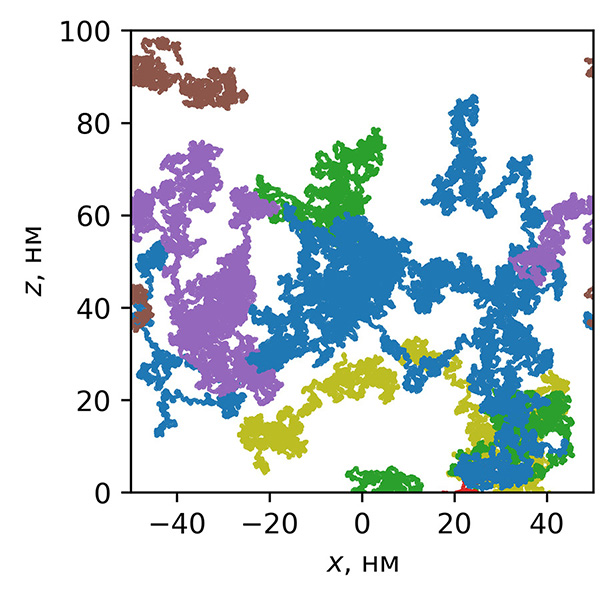
\includegraphics[width=0.95\linewidth]{G_value/Harris_chains_1step_200}
		\vspace{-14.2em} \\ \text{\hspace{0em} a}) \\ \vspace{14.2em}
	\end{minipage}
	\begin{minipage}{0.48\textwidth}
		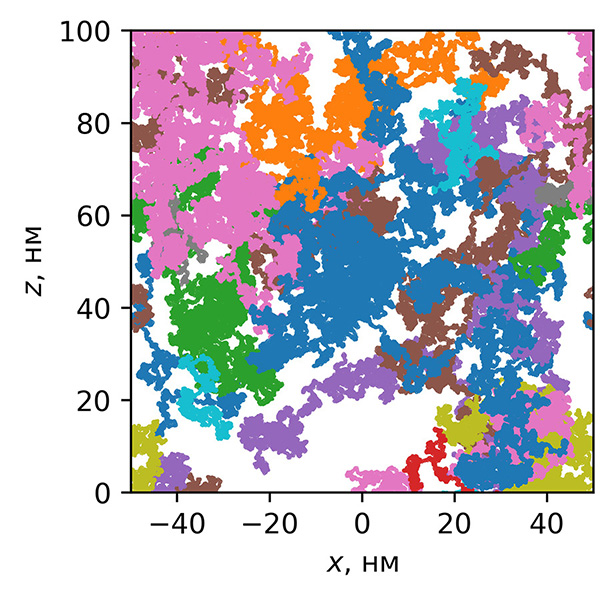
\includegraphics[width=0.95\linewidth]{G_value/Harris_chains_2step_200}
		\vspace{-14.2em} \\ \text{\hspace{0em} б}) \\ \vspace{14.2em}
	\end{minipage}
	\vspace{-3.5em}
	\begin{center}
		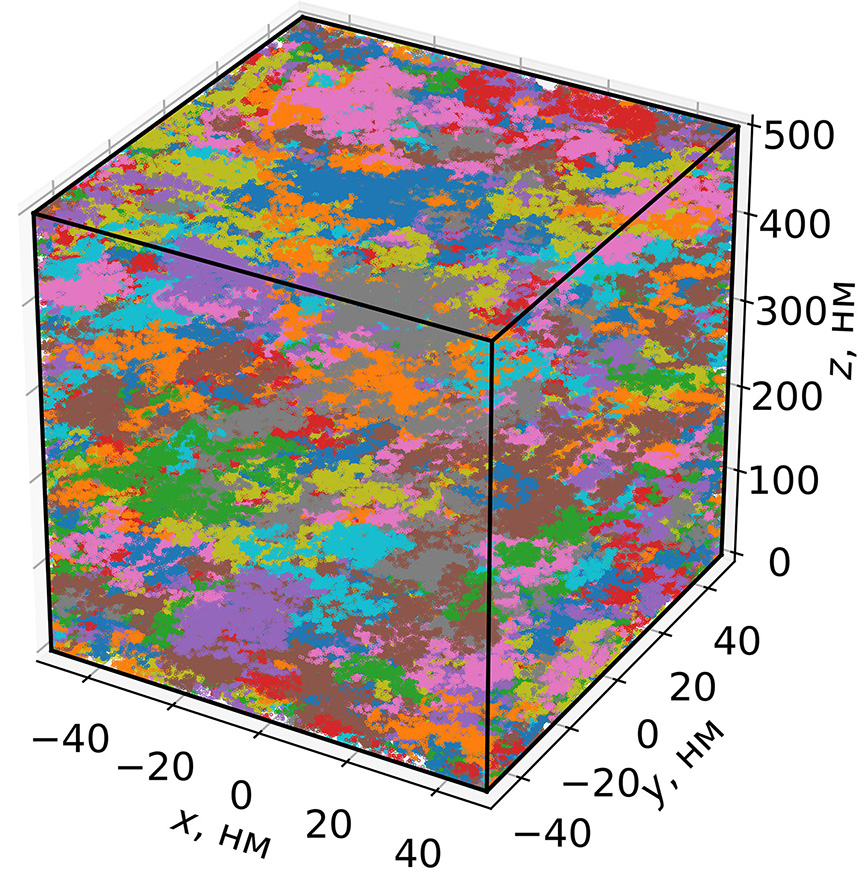
\includegraphics[width=0.5\linewidth]{G_value/Harris_chains_14_200}
		\vspace{-13em} \\ \text{\hspace{-20em} в}) \\ \vspace{13em}
	\end{center}
	\vspace{-1.5em}
	\caption{Иллюстрация процесса заполнения области моделями молекул ПММА (а, б) при моделировании слоя ПММА (в).}
	\label{fig:Harris_chains}
\end{figure}

Дальнейшее моделирование рассеяния электронного пучка в системе в системе ПММА/Si проводилось в предположении о равномерном распределении дозы экспонирования по площади для участка размерами 100$\times$100~нм$\pp$ с периодическими граничными условиями.
После этого область, занимаемая молекулами ПММА, разделялась на ячейки размерами 5$\times$5$\times$5 нм$\ppp$, и для каждой ячейки определялось соответствующее ей число промоделированных актов электрон-электронного рассеяния $N_{\mathrm{e-e}}[i, j, k]$.
Для каждого акта электрон-электронного рассеяния моделировалось, будет ли он приводить к разрыву молекулы ПММА или нет:
\begin{equation} \label{eq:MC_9}
	\begin{aligned}
		\xi < p_\mathrm{s} & \Rightarrow \text{разрыв молекулы} \\
		\xi \geq p_\mathrm{s} & \Rightarrow \text{нет разрыва},
	\end{aligned}
\end{equation}
где $\xi$ -- случайное число из промежутка [0, 1).
Таким образом, задание $p_\mathrm{s}$ позволяло промоделировать число разрывов в каждой ячейке слоя ПММА $N_\mathrm{s}[i, j, k]$.
Далее для каждой ячейки определялось, мономеры каких молекул находились в ней, и среди них случайным образом выбирались $N_\mathrm{s}[i, j, k]$ мономеров, которым сопоставлялись разрывы.
Учитывая тот факт, что номера молекул, проходящих через каждую ячейку, а также положения мономеров, входящих в каждую молекулу, хранились в памяти компьютера, такой подход позволял определить положения разрывов в каждой молекуле, входящей в модель слоя ПММА.
При известных положениях разрывов в каждой молекуле среднечисловая молекулярная масса проэкспонированного ПММА определялась непосредственным образом, и экспериментальное значение $\Gs$ рассчитывалось по формуле~\ref{eq:G_value_Mn_Mf}.

Экспериментальная зависимость $\Gs(T)$, приведенная в работе~\cite{Charlesby_1964_Gs}, была аппроксимирована функцией
\begin{equation}
	\ln(\Gs) = \frac{k}{T} + b,
\end{equation}
в результате чего были получены значения -454.012 и 2.008 для параметров $k$ и $b$ соответственно.
За счет этого были получены экспериментальные значения $\Gs$ для температур из диапазона 0--200~$^\circ$C, и для каждой температуры было подобрано значение $\ps$ обеспечивающее равенство между промоделированным и экспериментальным значениями $\Gs$ (``моделирование $\Gs$'' на рисунке~\ref{fig:P_s}).

Также, в качестве альтернативного подхода температурная зависимость $\ps$ была рассчитана непосредственно из определения $\Gs$ как числа разрывов, приходящегося на 100 эВ выделившейся в резисте энергии (``теоретическое $\Gs$'' на рисунке~\ref{fig:P_s}).
Явное различие между графиками, отображающими каждую из зависимостей, указывает на целесообразность моделирования молекулярно-массового распределения ПММА для определения $\ps$.

В таблице~\ref{table:p_s} приведены значения $\ps$, полученные для температур 130, 140 и 150~$^\circ$C при проведении пяти независимых моделирований.
Разброс значений для каждой температуры составляет менее 1\% от среднего значения, в силу чего было принято решение пренебречь статистической погрешностью $\ps$.

\begin{figure}[h]
	\centering
	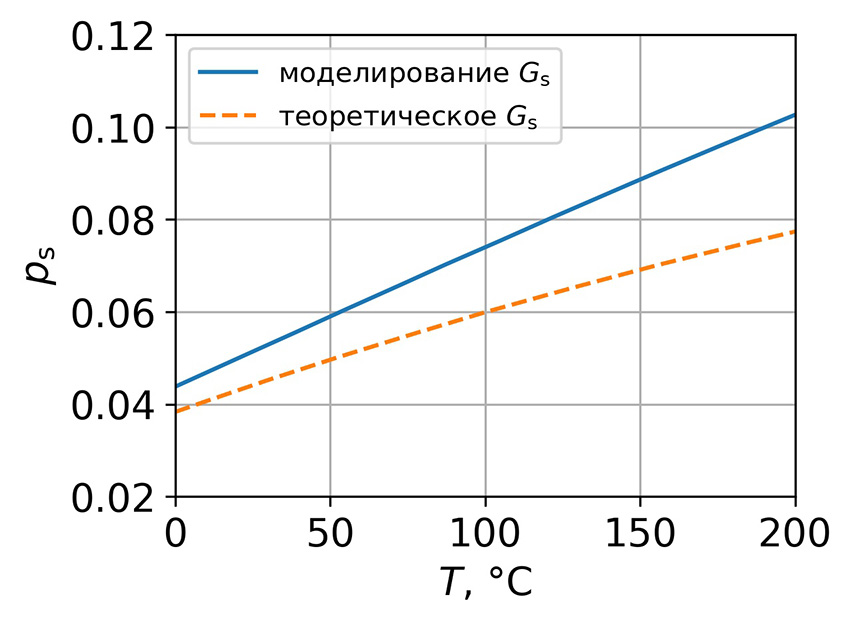
\includegraphics[width=0.55\linewidth]{G_value/G_s_14_200}
	\caption{Рассчитанная температурная зависимость вероятности разрыва $\ps$ молекулы ПММА при электрон-электронном взаимодействии (график ``моделирование $\Gs$''). График ``теоретическое $\Gs$'' отображает аналогичную зависимость, полученную непосредственно из определения величины $\Gs$.\vspace{1.5em}}
	\label{fig:P_s}
\end{figure}

\begin{table}[h]
	\caption{Значения вероятности разрыва молекулы ПММА при электрон-электронном взаимодействии для различных температур, полученные в пяти независимых моделированиях.}
	\begin{center}
		\begin{tabular}{c c r c r c r}
			\hline \hline \\[-1em]
			Номер моделирования & \hspace{0em} & $\ps$ при 130~$^\circ$C & \hspace{0em} & $\ps$ при 140~$^\circ$C & \hspace{0em} & $\ps$ при 150~$^\circ$C \\ \hline
			\\ [-1em]
			1 & \hspace{0em} & 8.2844\:$\cdot$\,10$^\text{-2}$ & \hspace{0em} & 8.5752\:$\cdot$\,10$^\text{-2}$ & \hspace{0em} & 8.8647\:$\cdot$\,10$^\text{-2}$
			\\ \\ [-1em]
			2 & \hspace{0em} & 8.3084\:$\cdot$\,10$^\text{-2}$ & \hspace{0em} & 8.6012\:$\cdot$\,10$^\text{-2}$ & \hspace{0em} & 8.8897\:$\cdot$\,10$^\text{-2}$
			\\ \\ [-1em]
			3 & \hspace{0em} & 8.2829\:$\cdot$\,10$^\text{-2}$ & \hspace{0em} & 8.5715\:$\cdot$\,10$^\text{-2}$ & \hspace{0em} & 8.8526\:$\cdot$\,10$^\text{-2}$
			\\ \\ [-1em]
			4 & \hspace{0em} & 8.2834\:$\cdot$\,10$^\text{-2}$ & \hspace{0em} & 8.5734\:$\cdot$\,10$^\text{-2}$ & \hspace{0em} & 8.8606\:$\cdot$\,10$^\text{-2}$
			\\ \\ [-1em]
			5 & \hspace{0em} & 8.2987\:$\cdot$\,10$^\text{-2}$ & \hspace{0em} & 8.5880\:$\cdot$\,10$^\text{-2}$ & \hspace{0em} & 8.8797\:$\cdot$\,10$^\text{-2}$
			\\ \hline \hline
		\end{tabular}
		\label{table:p_s}
	\end{center}
\end{table}

\section{Модель термической деполимеризации ПММА} \label{sec:depolymerization}

В данном разделе описывается подход, который был разработан для моделирования распределения среднечисловой молекулярной массы \linebreak ПММА в различные моменты процесса СЭЛТР.
Начальные значения среднечисловой ($\Mn$) и средневесовой ($\Mw$) молекулярной массы ПММА были приняты равными 271000 и 669000 соответственно, что соответствует резисту PMMA 950K A2 от компании <<Allresist>>, использовавшемуся в данной работе.
Предполагалось, что экспонирование производится ``в~кадр'' (вдоль серии параллельных линий), величина тока экспонирования была принята равной 5~нА, энергия электронного пучка -- 20 кэВ, размеры экспонируемой области -- \linebreak 2.4$\times$1.9 мм$\pp$, толщина слоя ПММА -- 500 нм, расстояние между линиями -- 3 мкм, время экспонирования -- 100 с, температура образца -- 130~$^\circ$C.
Данные значения согласуются со значениями соответствующих параметров в ранее проводившихся экспериментах по изучению метода СЭЛТР~\cite{Bruk_2016_mee}.
Число линий, получаемых при экспонировании ``в кадр'' составляет 625, однако для уменьшения требуемого машинного времени моделирование проводилось для участка одной линии длиной 100~нм с использованием периодических граничных условий.
На основе промоделированного распределения актов электрон-электронного взаимодействия в слое ПММА и вероятности разрыва (0.083 для 130~$^\circ$C) рассчитывалось распределение числа разрывов молекул ПММА.
$x-$ и $z-$координаты актов разрыва записывались в двумерную гистограмму с размером бина 50 нм по обеим осям.
Примеры гистограмм, отображающих распределение концентрации разрывов молекул ПММА при различных значений времени экспонирования, приведены на рисунке~\ref{fig:scission_hist}.

\begin{figure}[t]
	\begin{center}
		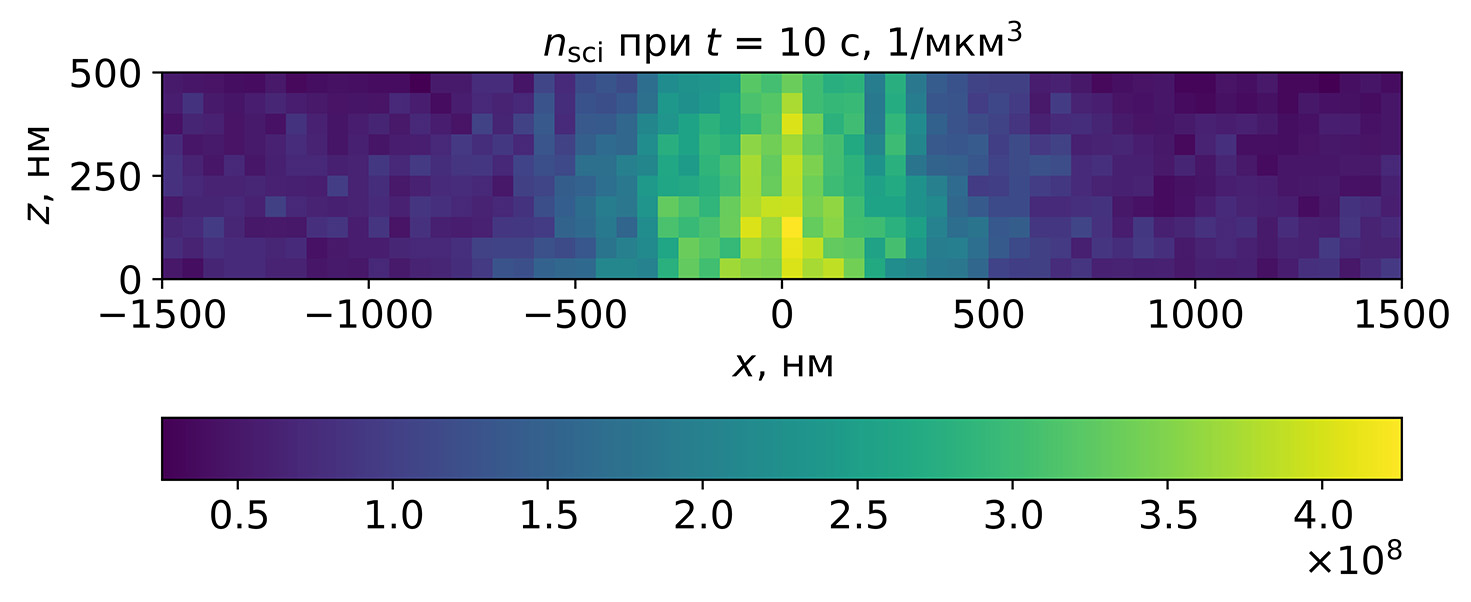
\includegraphics[width=0.8\linewidth]{MW/sci_conc_10s_straight_200} \\
		\vspace{-3.7em} \text{\hspace{-26em} a)} \vspace{2.7em} \\
		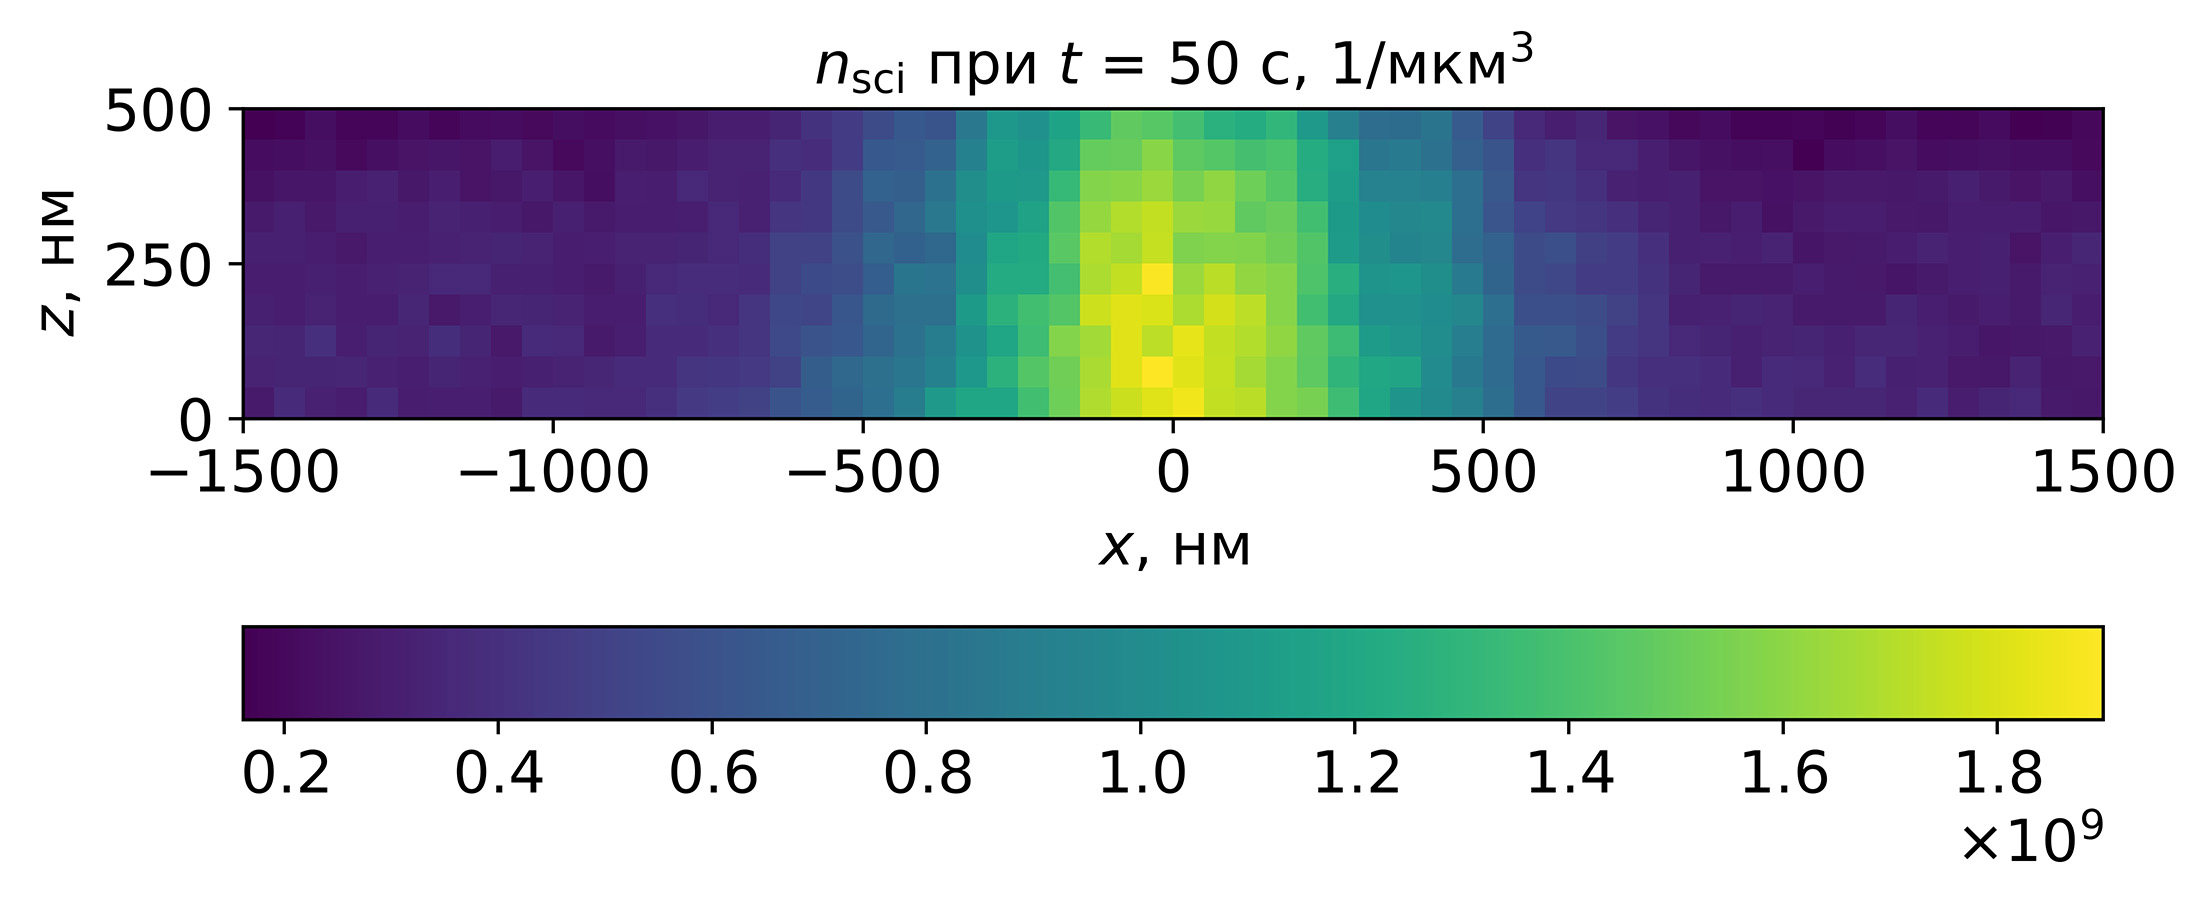
\includegraphics[width=0.8\linewidth]{MW/sci_conc_50s_straight_200} \\
		\vspace{-3.7em} \text{\hspace{-26em} б)} \vspace{3.7em} \\
	\end{center}
	\vspace{-2.5em}
	\caption{
		Промоделированные распределения концентрации разрывов молекул в слое ПММА при температуре 130~$^\circ$C.
		Экспонирование производилось ``в~кадр'', размеры кадра составляли 2.4$\times$1.9 мм$\pp$, число линий в кадре -- 625, расстояние между линиями -- 3 мкм, время экспонирования составляло 10 с (а) и 50 с (б).
		Энергия электронного пучка равна 20 кэВ, ток экспонирования -- 5~нА. Моделирование проводилось в пределах одной линии с периодическими граничными условиями.}
	\label{fig:scission_hist}
\end{figure}

Для моделирования молекулярно-массового распределения ПММА была использована модель, описанная в разделе~\ref{sec:depolymerization}.
Использовалось предположение о том, что молекулярно-массовое распределение ПММА описывается функцией распределения Шульца-Цимма со значениями среднечисловой и средневесовой молекулярной массы, равными 271000 и 669000 соответственно:
\begin{equation} \label{eq:Schulz-Zimm_distribution}
	P_n = C_0 n^z \exp (-n/y).
\end{equation}
Начальные значения параметров этого распределения ($z_0$ и $y_0$) были найдены на основе формул \ref{eq:Schulz-Zimm_1} и \ref{eq:Schulz-Zimm_2}:
\begin{equation}
	\begin{aligned}
		PD & \equiv \frac{\Mw}{\Mn} = \frac{669000}{271000} \cong 2.47, \\
		z_0 & = (2-PD)/(PD-1) \cong -0.32, \\
		y_0 & = x_0/(z_0+1) \cong 3989.58.
	\end{aligned}
\end{equation}
Также, согласно результатам работы~\cite{Mita_PMMA_zip_lengths_T}, средняя длина цепи деполимеризации при 130~$^\circ$C была принята равной 500.
После задания всех параметров система дифференциальных уравнений~\ref{eq:scary_system} решалась численно методом Рунге-Кутты 4 порядка с переходом на схему предиктор-корректор начиная с четвертого шага (рисунок~\ref{fig:SZ_M1_y_tau}).
Диапазон значений переменной $\tau$ составлял от 0 до 400 с шагом 0.01.
\begin{figure}[t]
	\begin{minipage}{0.48\textwidth}
			\hspace{-0.5em} 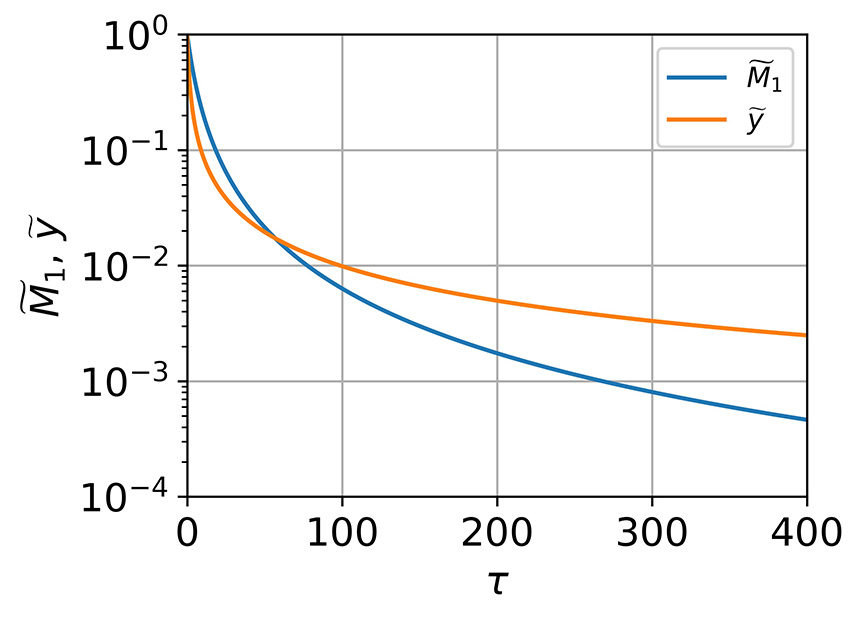
\includegraphics[width=\linewidth]{MW/SZ_M1_y_14_200} \\
			\vspace{-12.5ex} \\ \text{\hspace{3.8em} a}) \\ \vspace{12.5ex}
		\end{minipage}
	\begin{minipage}{0.48\textwidth}
			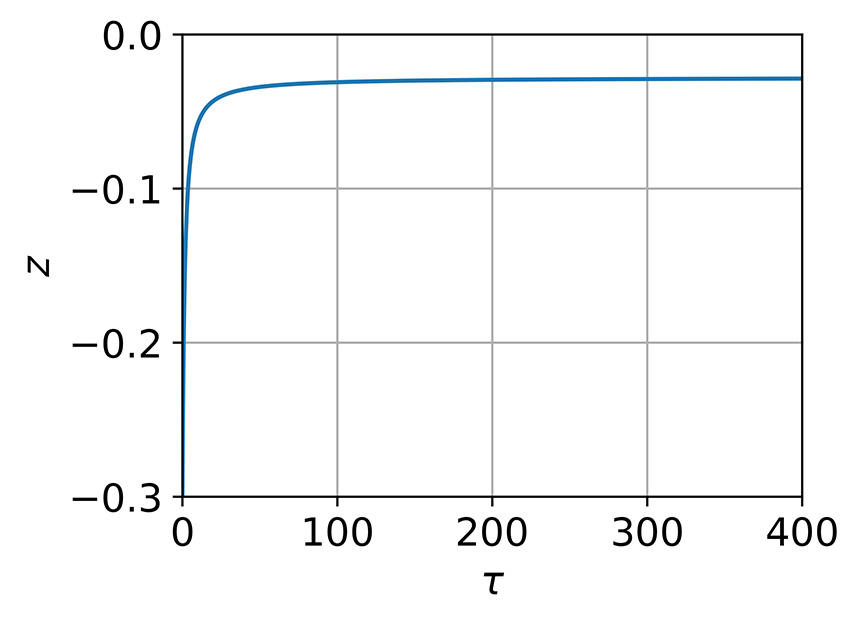
\includegraphics[width=\linewidth]{MW/SZ_z_14_200} \\
			\vspace{-12.5ex} \\ \text{\hspace{4em} б}) \\ \vspace{12.5ex}
		\end{minipage}
	\vspace{-3.5em}
	\caption{
		Зависимости параметров распределения Шульца-Цимма $\tilde{M_1}$, $\tilde{y}$ (а) и $z$ (б) от безразмерной временной переменной $\tau$, полученные для резиста PMMA 950K A2, использовавшегося в данной работе.
	}
	\label{fig:SZ_M1_y_tau}
\end{figure}
Зависимости параметров распределения молекулярной массы резиста от безразмерной переменной $\tau$ далее пересчитывались в зависимости от времени экспонирования $t$ по формуле~\ref{eq:dim_less_MW}:
\begin{equation} \label{eq:tau_y0_ks_t}
	\tau = y_0 k_\mathrm{s} t.
\end{equation}

Входящая в это выражение величина $k_\mathrm{s}$, выражающая число активных центров деполимеризации, появляющихся за 1 с, приходящееся на один мономер, определялась следующим образом.
Изначально была создана двумерная гистограмма с размерами, аналогичными размерам гистограммы для распределения числа разрывов, в каждую ячейку которой (условно с индексами $i$ и $j$) в качестве начального значения величины $\tau$ было записано число 0.
Далее для каждой секунды экспонирования моделировалось число разрывов молекул ПММА, относившихся к этой ячейке ($N_\mathrm{sci}^\mathrm{1c}[i,j]$).
При этом считалось, что число активных центров деполимеризации, появлявшихся за 1 с в данной ячейке, равнялось числу промоделированных разрывов полимерных молекул в ячейке.
После этого прибавка к величине $\tau$ в данной ячейке, соответствующая 1 секунде экспонирования, определялась по формуле~\ref{eq:tau_y0_ks_t}:
\begin{equation}
	\Delta \tau_\mathrm{1c} [i,j] = 3989.58 \cdot \frac{N_\mathrm{sci}^\mathrm{1c}[i,j]}{1789618} \cdot 1с,
\end{equation}
где 1789618 -- число мономеров в одной ячейке гистограммы (область размерами 50$\times$100$\times$50 нм$\ppp$), рассчитанное на основе плотности ПММА и молярной массы ММА (1.19~г/см$\ppp$ и 100 г/моль соответственно).
Величина $\Delta \tau_\mathrm{1c} [i,j]$ добавлялась к текущему значению $\tau$ для данной ячейки и далее для нового значения $\tau$ определялись соответствующие значения параметров $y$ и $z$ молекулярно-массового распределения ПММА.
Такой подход позволял вычислить локальные значения среднечисловой массы ПММА в различные моменты времени экспонирования по формуле
\begin{equation}
	M_\mathrm{n} [i,j] (t) = y[i,j] (t) (z [i,j] (t) + 1).
\end{equation}
Промоделированные таким образом пространственные распределения локальной среднечисловой молекулярной массы ПММА для двух различных значений времени экспонирования приведены на рисунке~\ref{fig:Mn_hist}.

\begin{figure}[h]
	\begin{center}
		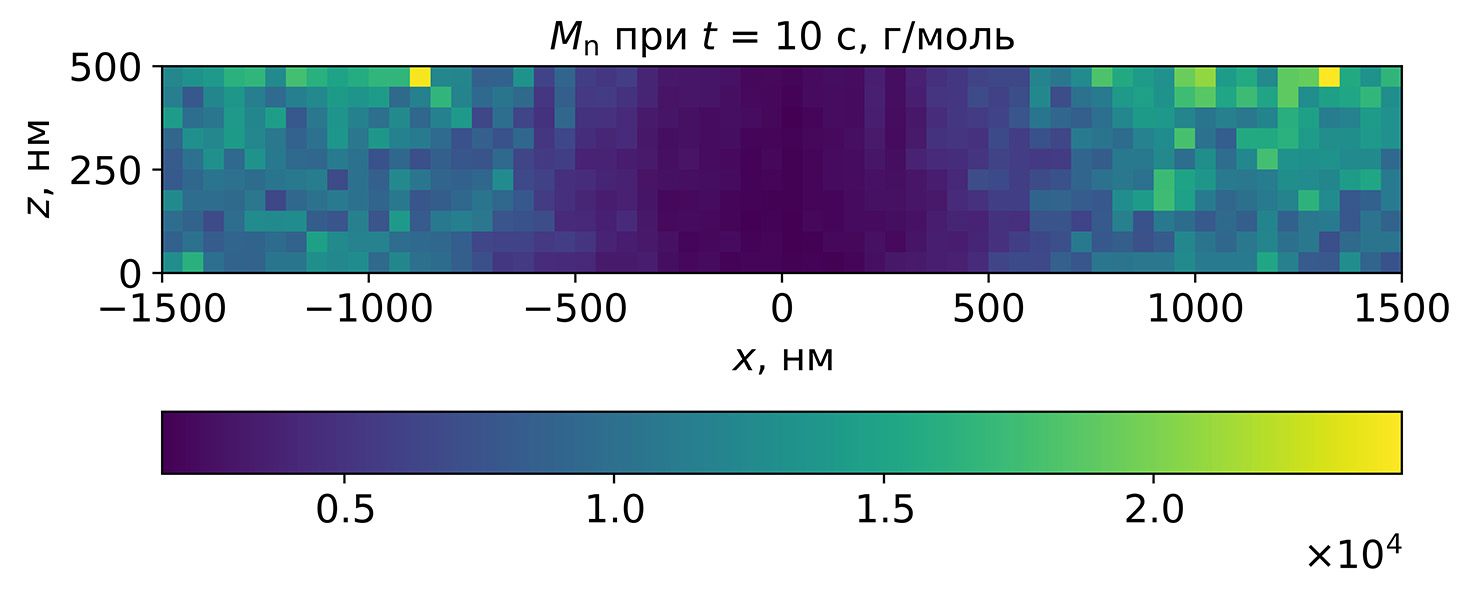
\includegraphics[width=0.8\linewidth]{MW/Mn_hist_10s_straight_200} \\
		\vspace{-3.7em} \text{\hspace{-26em} a)} \vspace{2.7em} \\
		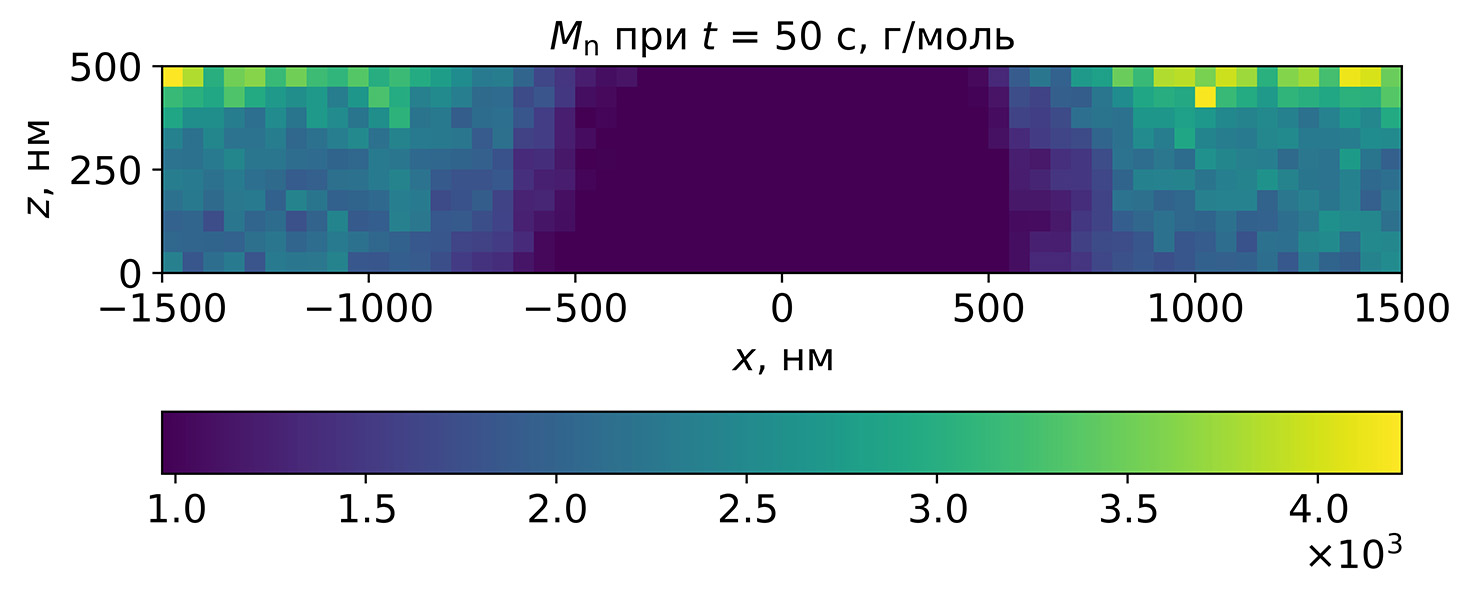
\includegraphics[width=0.8\linewidth]{MW/Mn_hist_50s_straight_200} \\
		\vspace{-3.7em} \text{\hspace{-26em} б)} \vspace{3.7em} \\
	\end{center}
	\vspace{-2.5em}
	\caption{
		Промоделированные распределения локальной среднечисловой молекулярной массы PMMA 950К A2 при температуре 130~$^\circ$C.
		Экспонирование производилось ``в~кадр'', размеры кадра составляли 2.4$\times$1.9 мм$\pp$, число линий в кадре -- 625, расстояние между линиями -- 3 мкм, время экспонирования составляло 10 с (а) и 50 с (б).
		Энергия электронного пучка равна 20 кэВ, ток экспонирования -- 5~нА. Моделирование проводилось в пределах одной линии с периодическими граничными условиями.}
	\label{fig:Mn_hist}
\end{figure}

\section{Модель диффузии мономера в слое ПММА}

Оценка времени диффузии мономера, образующегося в слое ПММА в процессе СЭЛТР, проводилась на основе значений коэффициента диффузии, приведенных в работе~\cite{Karlsson2001_diffusion} (среднечисловая молекулярная масса ПММА в этой работе составляла примерно 30000). Для получения оценки для времени диффузии сверху была рассмотрена минимальная из температур -- 135~$^\circ$C.
Исходное значение коэффициента диффузии ММА в ПММА при 135~$^\circ$C (2\:$\cdot$\,10$^\text{-10}$ см$\pp$/с) было пересчитано для резиста PMMA 950K A2 со среднечисловой молекулярной массой около 271000, использовавшегося в данной работе, по формуле~\ref{eq:diffusion_Mn}:
\begin{equation}
	\begin{cases}
		\lg D_{30000} = \lg D_{\infty} + \displaystyle{\frac{k}{30000}}, \vspace{0.4em} \\
		\lg D_{271000} = \lg D_{\infty} + \displaystyle{\frac{k}{270000}},
	\end{cases}
\end{equation}
где $k$ = 1.06\:$\cdot$\,10$^\text{4}$. Это приводит к следующему выражению для коэффициента диффузии ММА в ПММА при 135~$^\circ$C (в см$\pp$/с):
\begin{equation}
	D_{271000}^{135 \, ^\circ \mathrm{C}} = D_{30000} \cdot 10^{k \left(\frac{1}{271000} - \frac{1}{30000} \right)} = 2 \cdot 10^{-10} \cdot 10^{1.06 \cdot 10^4 \left(\frac{1}{271000} - \frac{1}{30000} \right)} \cong 9.7 \cdot 10^{-11}.
\end{equation}
При экспонировании локальная молекулярная масса ПММА уменьшается, что приводит к увеличению коэффициента диффузии. Согласно формуле~\ref{eq:diffusion_Mn}, коэффициент диффузии ММА в ПММА (в см$\pp$/с) для ПММА со среднечисловой молекулярной массой $M_\mathrm{n}$ < 271000 при температуре 135~$^\circ$C может быть рассчитан следующим образом (рисунок~\ref{fig:Mn_diff}):
\begin{equation} \label{eq:D_Mn}
	D_{\Mn}^{135 \, ^\circ \mathrm{C}} = 9.7 \cdot 10^{-11} \cdot 10^{1.06 \cdot 10^4 \left( \frac{1}{271000} - \frac{1}{\Mn} \right)}.
\end{equation}

\begin{figure}[h]
	\begin{center}
		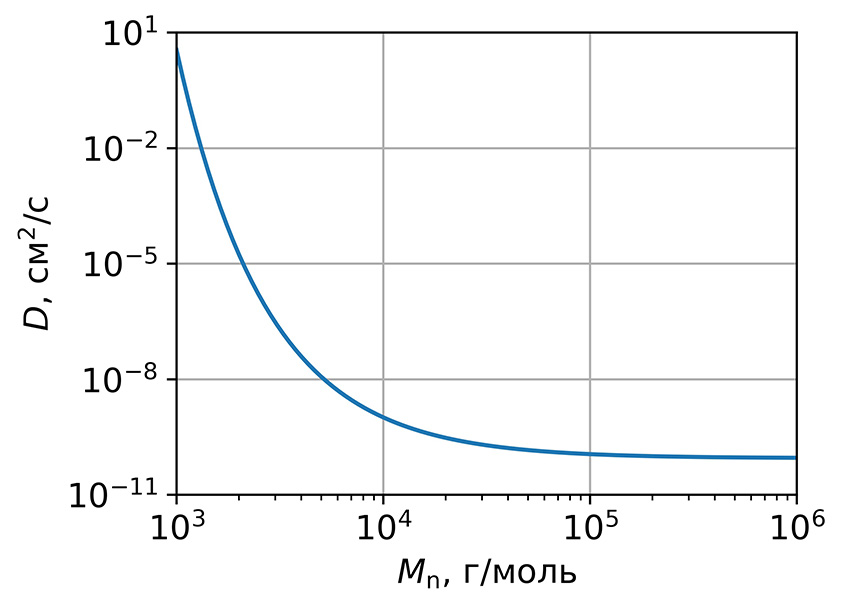
\includegraphics[width=0.55\linewidth]{diffusion/DD_12_straight_200}
	\end{center}
	\vspace{-1em}
	\caption{Зависимость коэффициента диффузии ММА в ПММА ($D$) от среднечисловой молекулярной массы ПММА ($\Mn$) при 135~$^\circ$C.}
	\label{fig:Mn_diff}
\end{figure}

Для оценки времени выхода мономера из слоя ПММА проводилось численное решение уравнения диффузии для мономера, образовавшегося в слое ПММА за 1~секунду в процессе СЭЛТР с параметрами экспонирования, описанными в разделе~\ref{sec:depolymerization}.
Начальное распределение количества свободного мономера в слое ПММА определялось за счет умножения промоделированного распределения числа разрывов молекул ПММА, произошедших за 1~секунду экспонирования, на среднюю длину кинетической цепи при деполимеризации (принятую равной 500 для температуры 135~$^\circ$C).
Далее время выхода мономера из слоя \linebreak ПММА оценивалось как время, за которое концентрация мономера в центре линии уменьшалась в 10 раз.
При коэффициенте диффузии, равном 9.7\:$\cdot$\,10$^\text{-11}$~см$\pp$/c, это время составляет около 15 с (рисунок~\ref{fig:diffusion_initial}).
Однако, уже после 10 секунд экспонирования среднечисловая молекулярная масса резиста на краях линии снижается до значений порядка 1\:$\cdot$\,10$^\text{4}$, что соответствует значению коэффициента диффузии около 1\:$\cdot$\,10$^\text{-9}$ см$\pp$/c.
В этом случае время, за которое концентрация мономера в центре линии уменьшается в 10 раз составляет около 1 с (рисунок~\ref{fig:diffusion_10s}).

В вышеописанных расчетах использовался коэффициент диффузии на краях линии, в центре линии (где молекулярная масса резиста в разы меньше (рисунок~\ref{fig:Mn_hist}) значение коэффициента диффузии будет выше согласно формуле~\ref{eq:D_Mn}.
Принимая также во внимание тот факт, что данные расчеты относятся к минимальной из температур, при которых проводились эксперименты по исследованию метода СЭЛТР, можно заключить, что временем диффузии мономера из слоя ПММА в процессе СЭЛТР можно пренебречь по сравнению с характерным временем экспонирования.
Поэтому в дальнейшем будет считаться, что весь свободный мономер, образующийся в процессе деполимеризации, мгновенно покидает слой ПММА.

%Это также подтверждает предположения о быстрой диффузии мономера, сделанные в работе~\cite{Bruk_2013} на основе формулы для времени диффузионного проскока молекул газа через слой толщины $l$:
%\begin{equation} \label{eq:Bruk_tau_diff}
%	\tau_{\text{diff}} = \frac{l^2}{12 D_\mathrm{e}},
%\end{equation}
%где $D_\mathrm{e}$ -- эффективный коэффициент диффузии газа.
%При толщине слоя 500 нм и значении коэффициента диффузии 9.7\:$\cdot$\,10$^\text{-11}$ см$\pp$/с время $\tau_{\text{diff}}$, вычисленное по формуле~\ref{eq:Bruk_tau_diff} составляет около 2 с.

%В силу полученных оценок для времени диффузии мономера из слоя \linebreak ПММА в дальнейшем будет считаться, что свободный мономер, образующийся в процессе деполимеризации, мгновенно покидает слой ПММА.

\begin{figure}[H]
	\begin{center}
		\vspace{-1em}
%		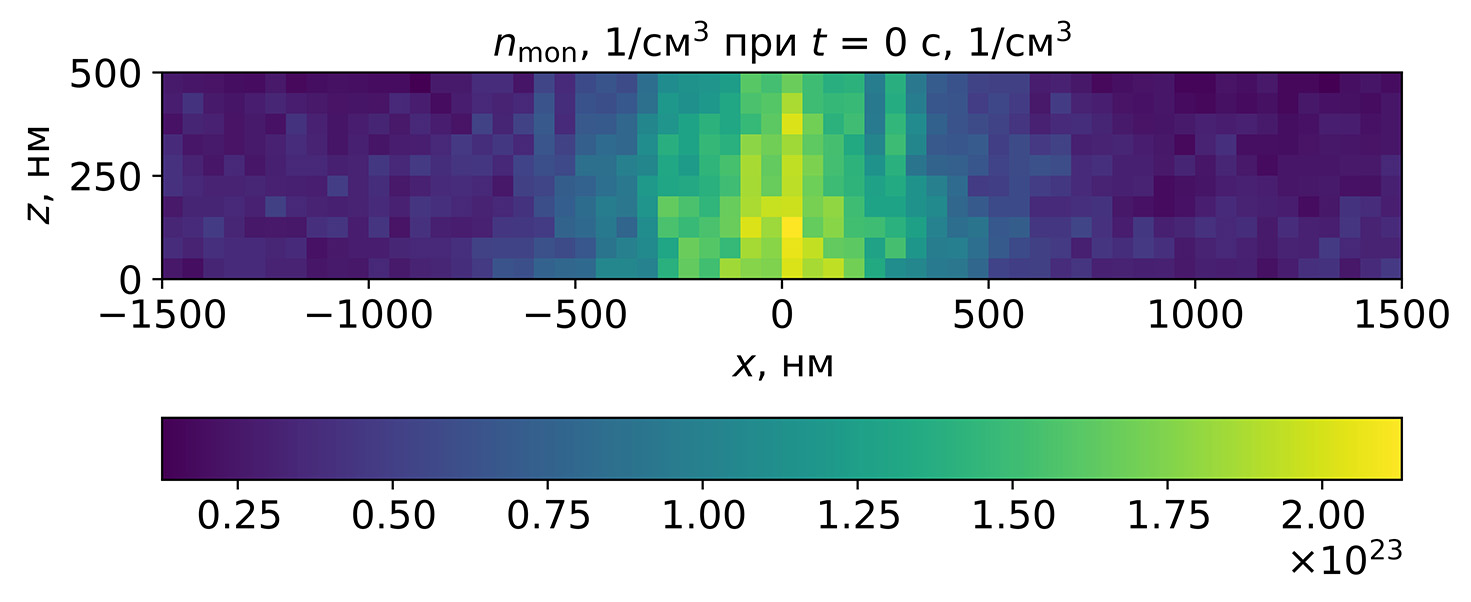
\includegraphics[width=0.8\linewidth]{diffusion/n_mon_initial_straight_200} \\
%		\vspace{-4em} \text{\hspace{-26em} a)} \vspace{2.2em} \\
%		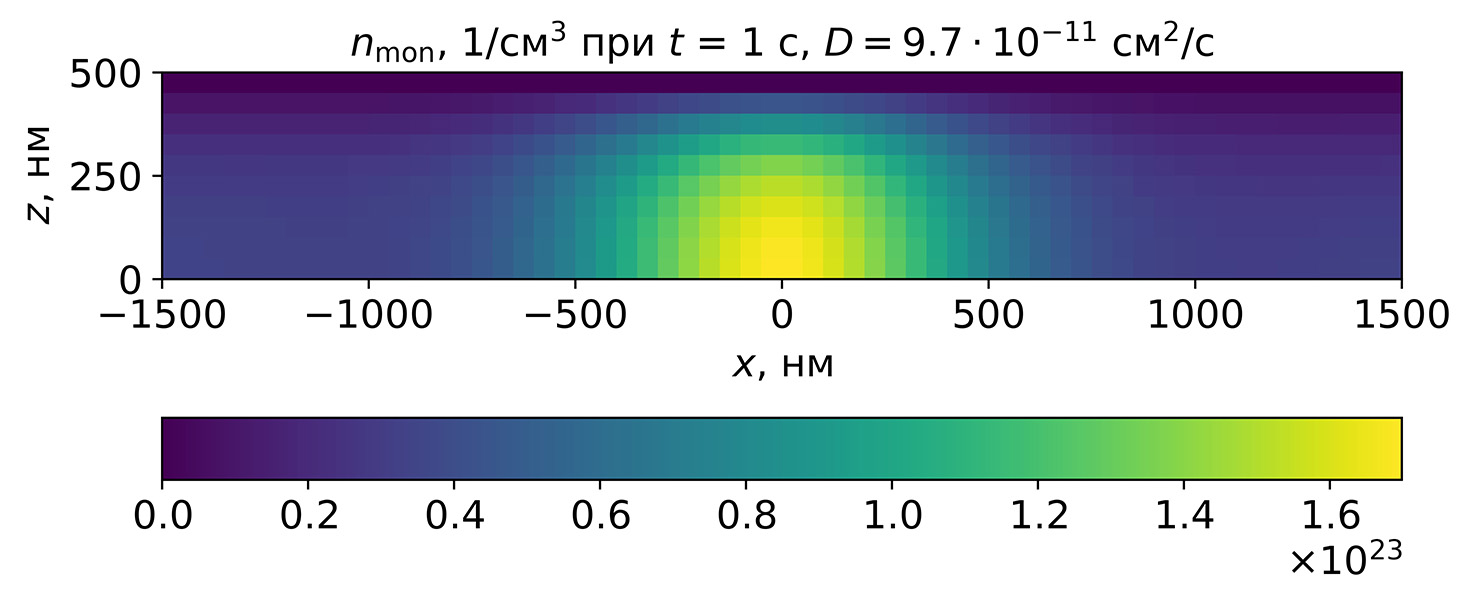
\includegraphics[width=0.8\linewidth]{diffusion/n_mon_9p7e-11_1s_straight_200} \\
%		\vspace{-4em} \text{\hspace{-26em} б)} \vspace{2.2em} \\
%		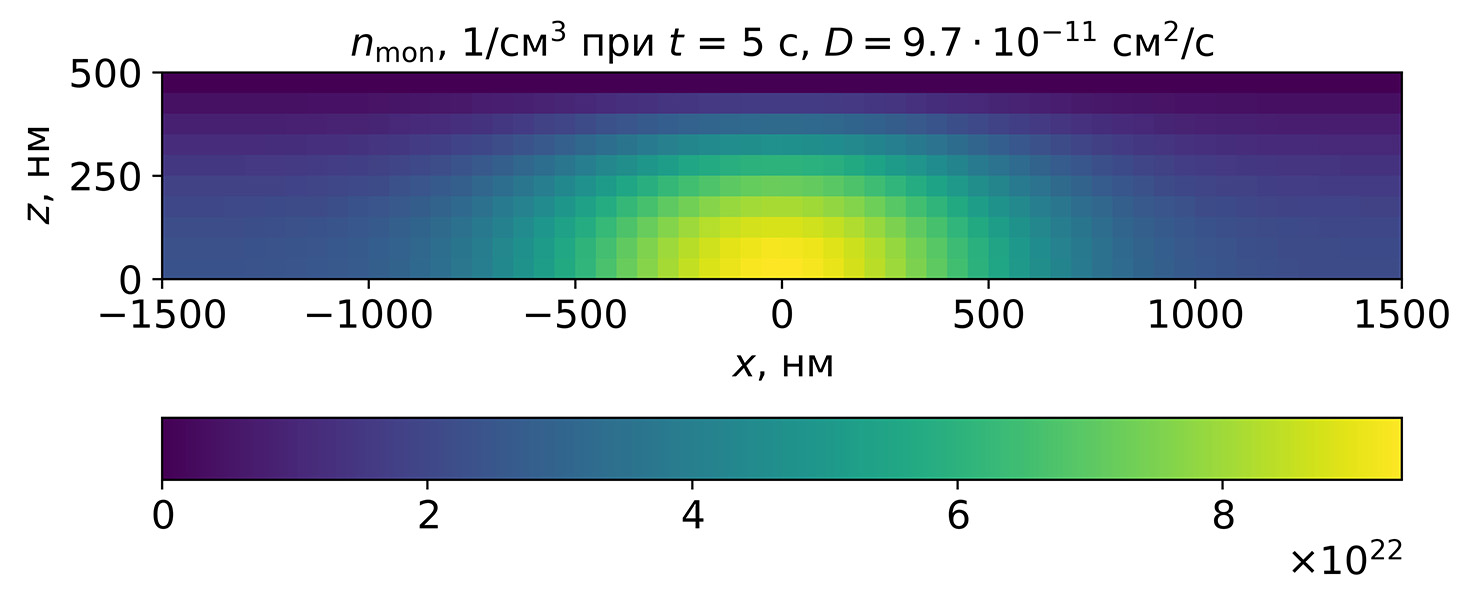
\includegraphics[width=0.8\linewidth]{diffusion/n_mon_9p7e-11_5s_straight_200} \\
%		\vspace{-4em} \text{\hspace{-26em} в)} \vspace{2.2em} \\
%		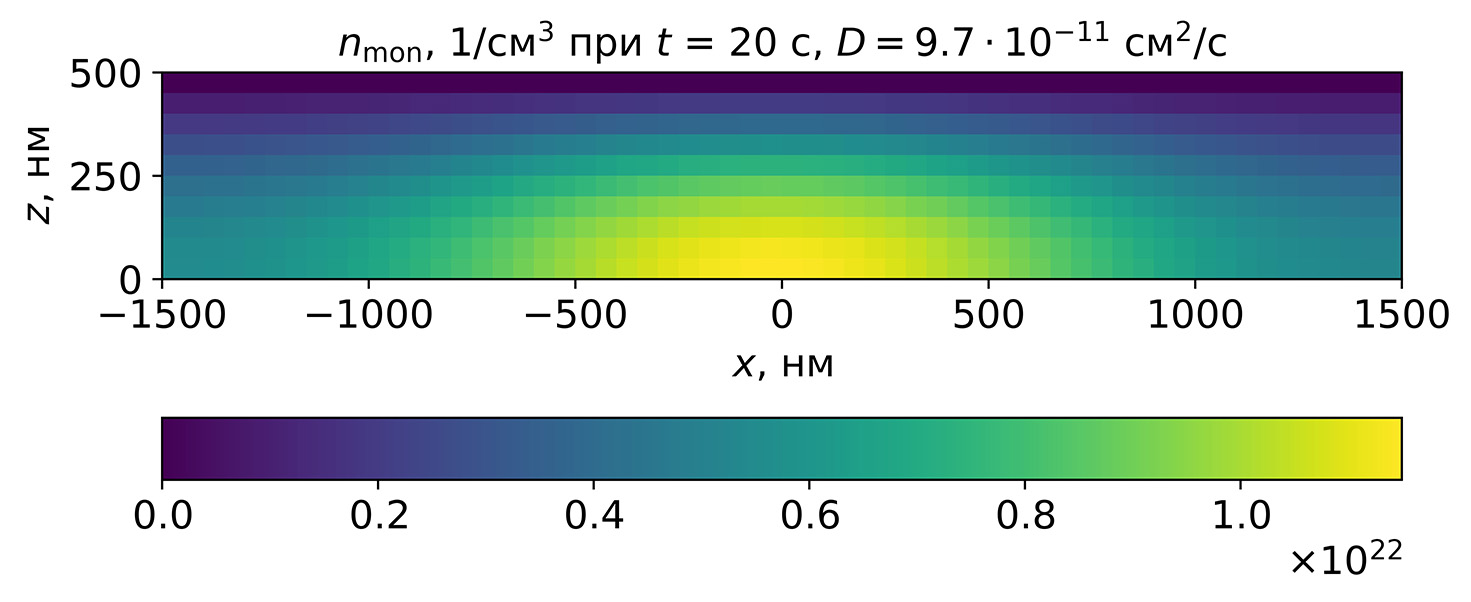
\includegraphics[width=0.8\linewidth]{diffusion/n_mon_9p7e-11_20s_straight_200} \\
%		\vspace{-4em} \text{\hspace{-26em} г)} \vspace{2.2em} \\
		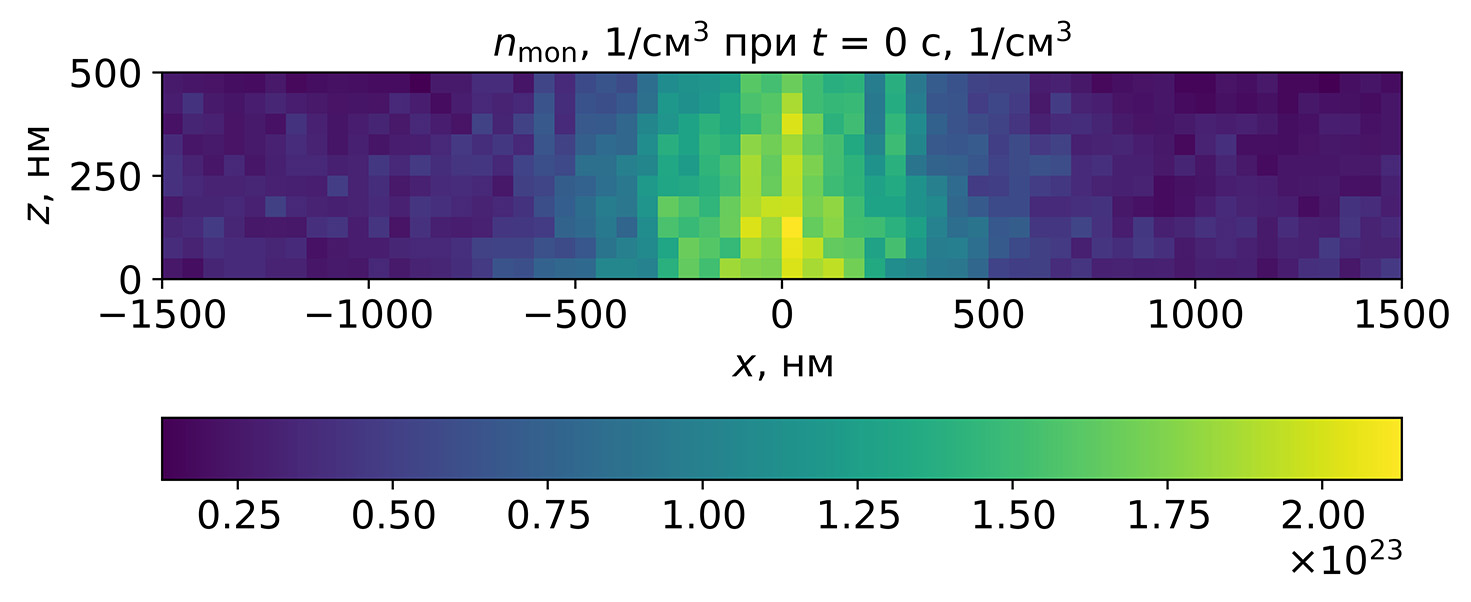
\includegraphics[width=0.8\linewidth]{diffusion/n_mon_initial_straight_200} \\
		\vspace{-4em} \text{\hspace{-26em} a)} \vspace{2em} \\
		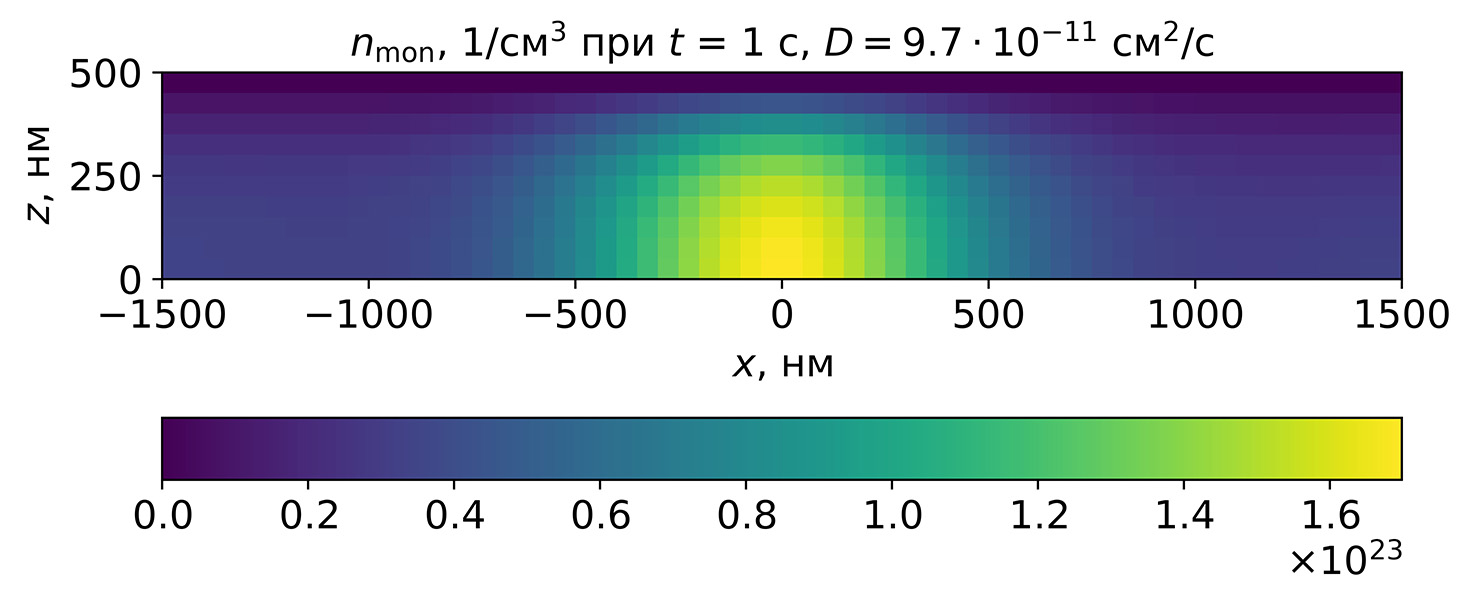
\includegraphics[width=0.8\linewidth]{diffusion/n_mon_9p7e-11_1s_straight_200} \\
		\vspace{-4em} \text{\hspace{-26em} б)} \vspace{2em} \\
		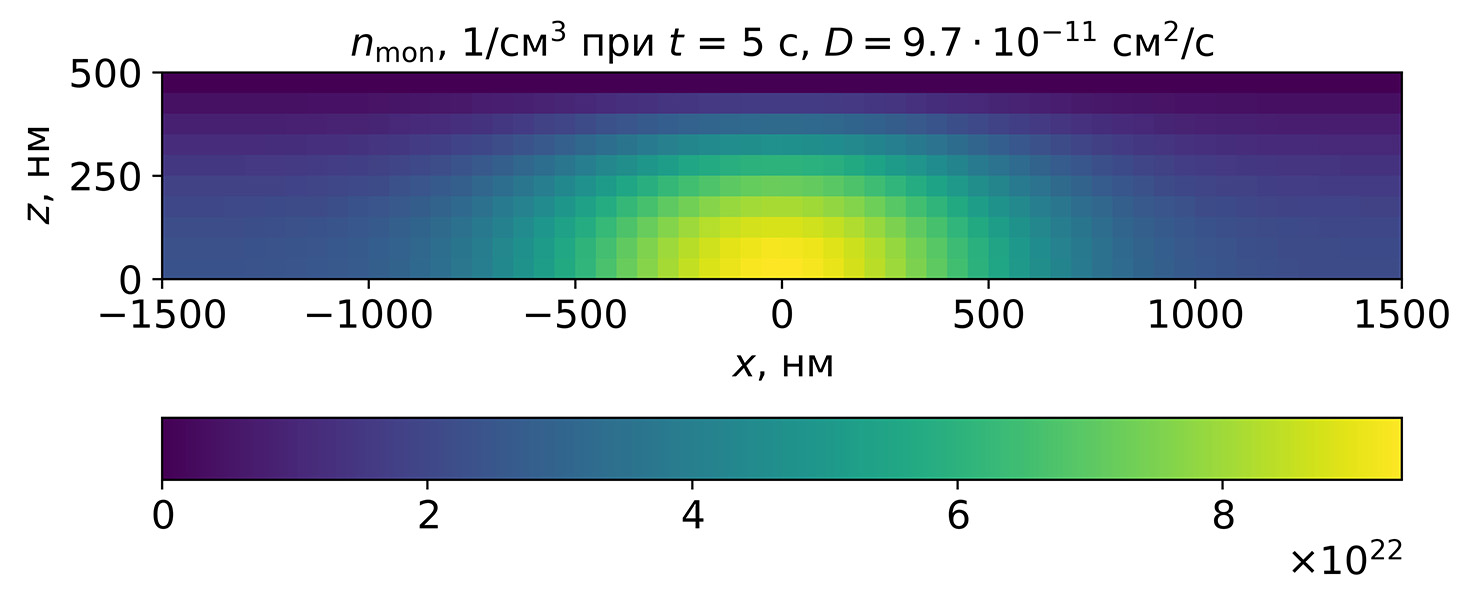
\includegraphics[width=0.8\linewidth]{diffusion/n_mon_9p7e-11_5s_straight_200} \\
		\vspace{-4em} \text{\hspace{-26em} в)} \vspace{2em} \\
		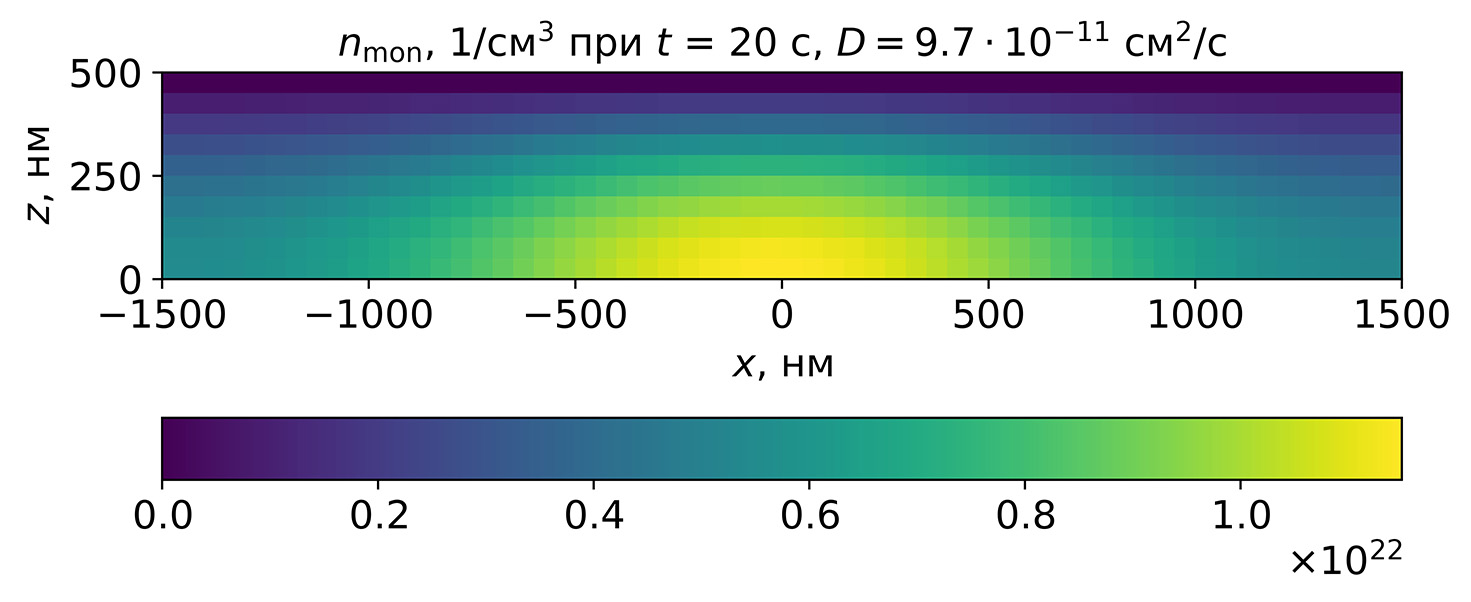
\includegraphics[width=0.8\linewidth]{diffusion/n_mon_9p7e-11_20s_straight_200} \\
		\vspace{-4em} \text{\hspace{-26em} г)} \vspace{2em} \\
	\end{center}
%	\vspace{-1em}
	\vspace{-1.5em}
	\caption{Моделирование диффузии мономера, образовавшегося в слое ПММА за 1~секунду в процессе СЭЛТР при температуре 135~$^\circ$C с параметрами экспонирования, описанными в разделе~\ref{sec:depolymerization}: а) начальное распределение концентрации мономера; б), в), г) распределения концентрации мономера после диффузии в течение 1, 5 и 20 с соответственно. Коэффициент диффузии составляет 9.7\:$\cdot$\,10$^\text{-11}$ см$\pp$/c.}
	\label{fig:diffusion_initial}
\end{figure}

\newpage

\begin{figure}[H]
	\begin{center}
		\vspace{-1em}
%		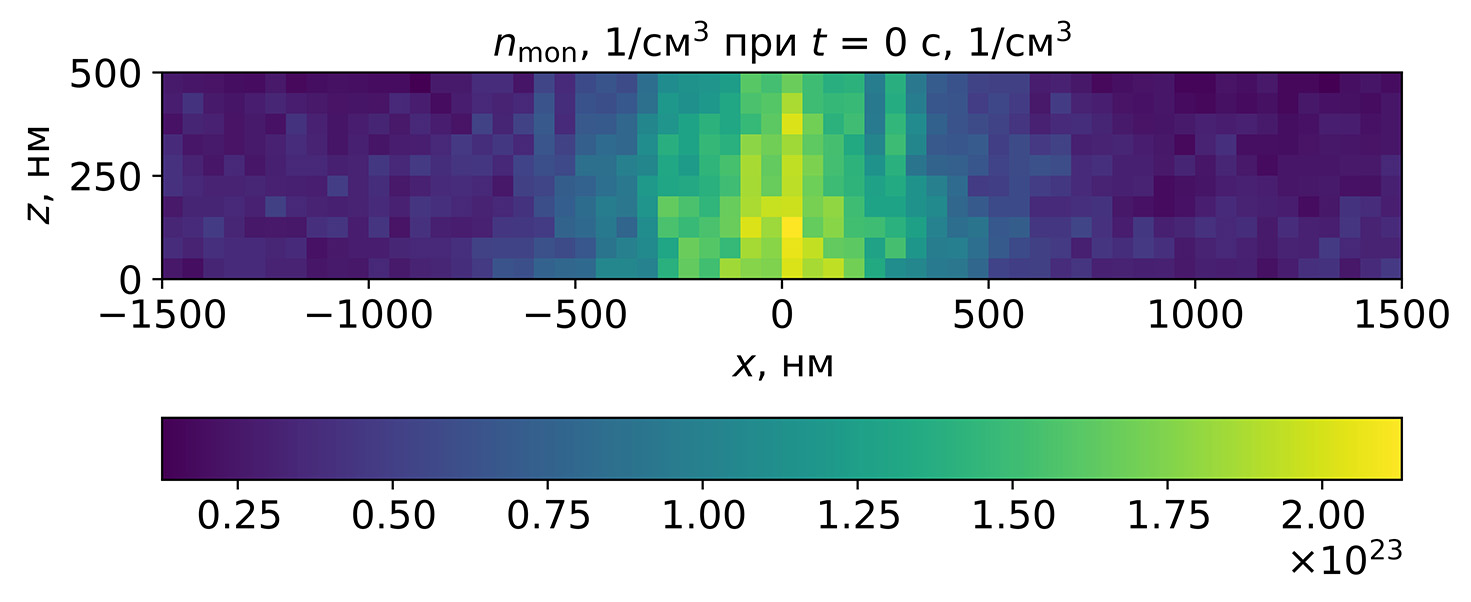
\includegraphics[width=0.8\linewidth]{diffusion/n_mon_initial_straight_200} \\
%		\vspace{-4em} \text{\hspace{-26em} a)} \vspace{2.2em} \\
%		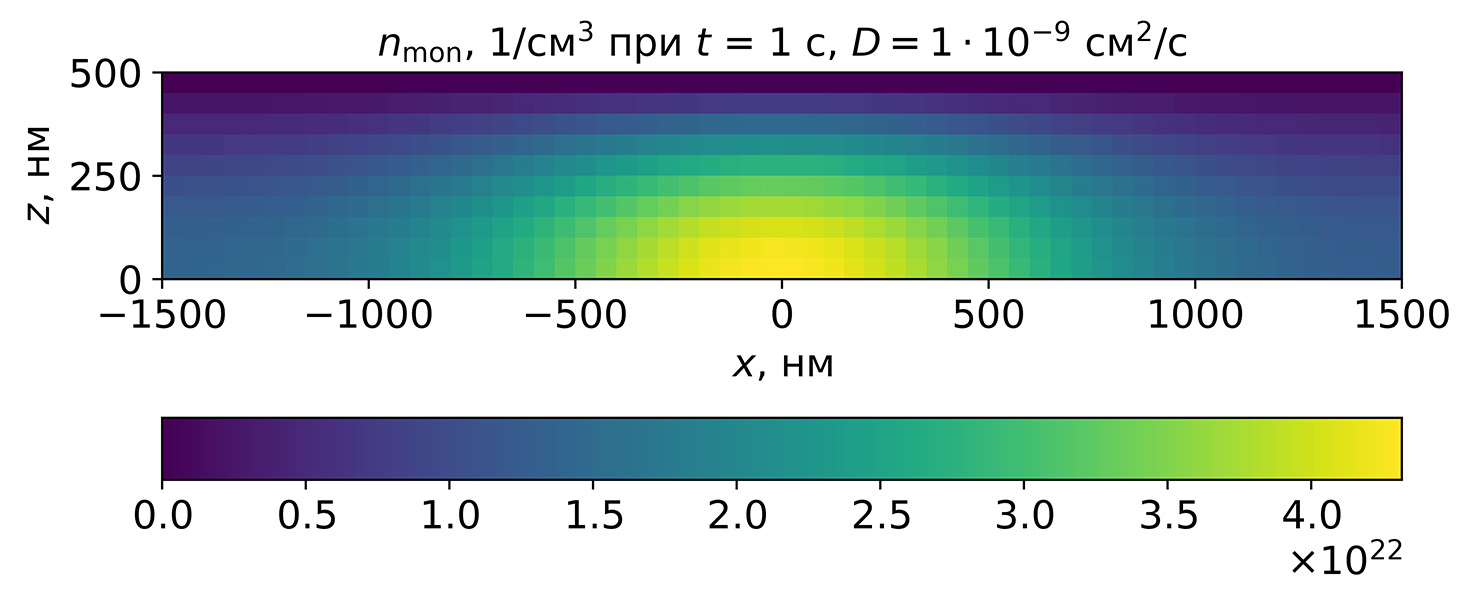
\includegraphics[width=0.8\linewidth]{diffusion/n_mon_1e-9_1s_straight_200} \\
%		\vspace{-4em} \text{\hspace{-26em} б)} \vspace{2.2em} \\
%		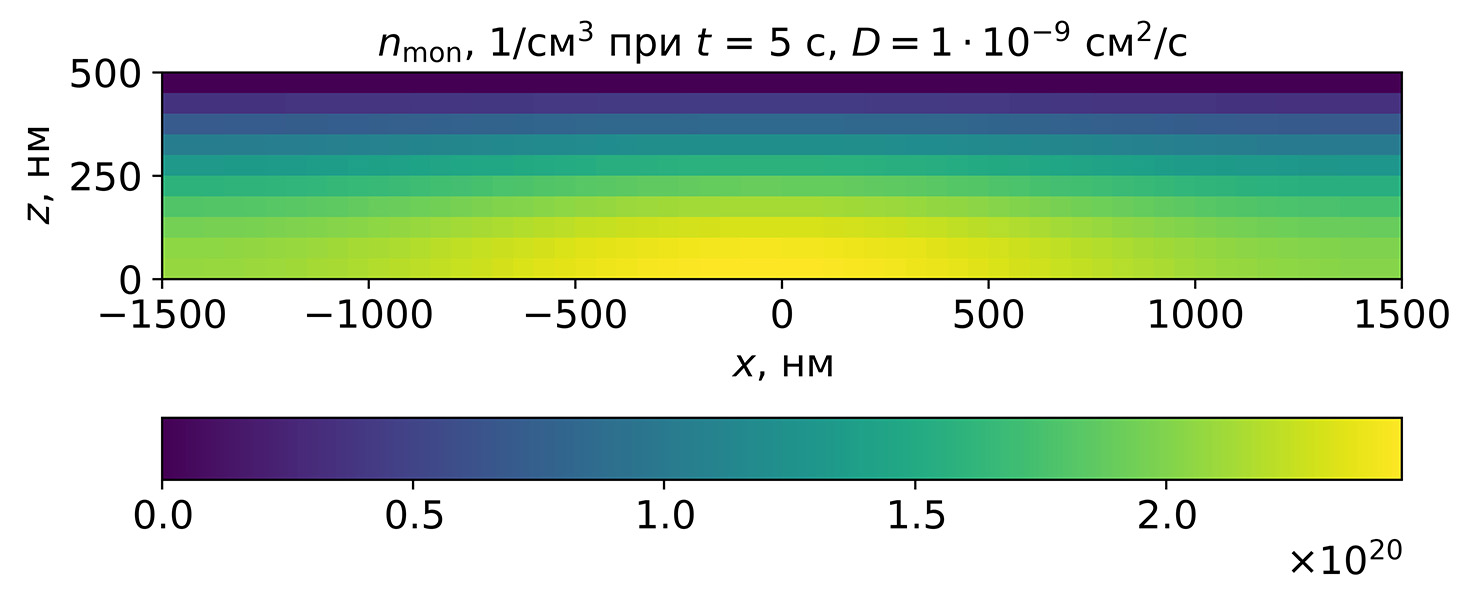
\includegraphics[width=0.8\linewidth]{diffusion/n_mon_1e-9_5s_straight_200} \\
%		\vspace{-4em} \text{\hspace{-26em} в)} \vspace{2.2em} \\
%		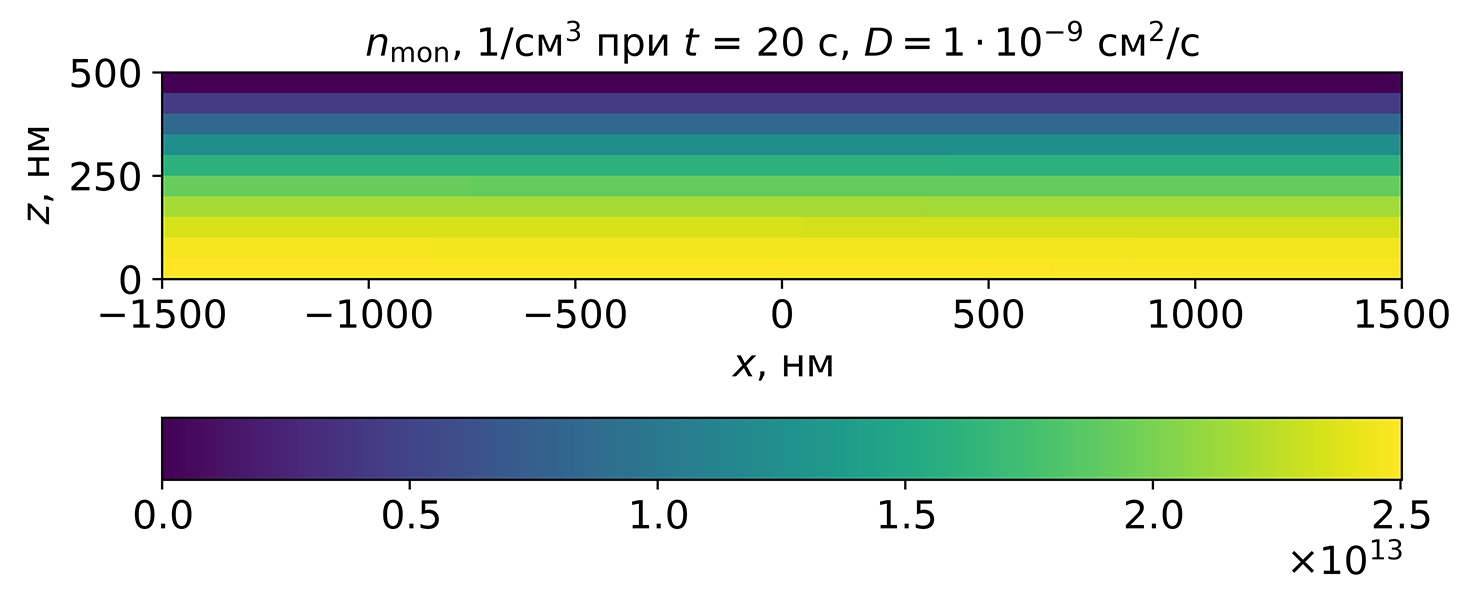
\includegraphics[width=0.8\linewidth]{diffusion/n_mon_1e-9_20s_straight_200} \\
%		\vspace{-4em} \text{\hspace{-26em} г)} \vspace{2.2em} \\
		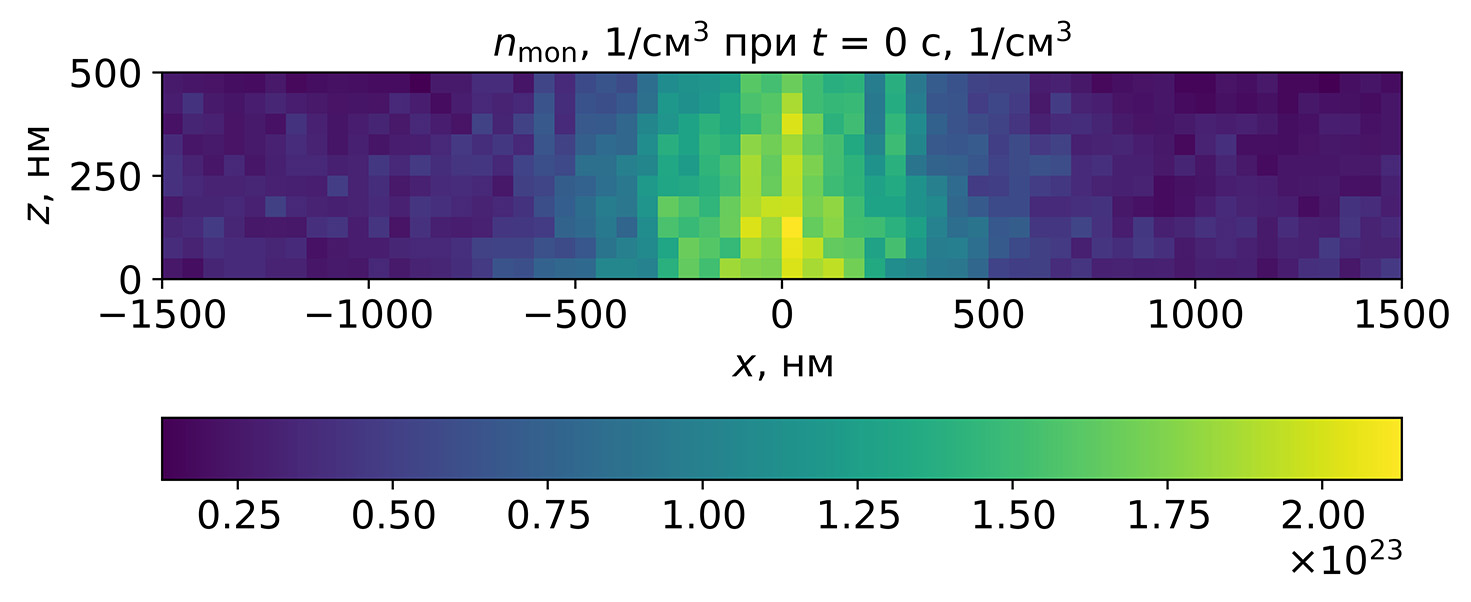
\includegraphics[width=0.8\linewidth]{diffusion/n_mon_initial_straight_200} \\
		\vspace{-4em} \text{\hspace{-26em} a)} \vspace{2em} \\
		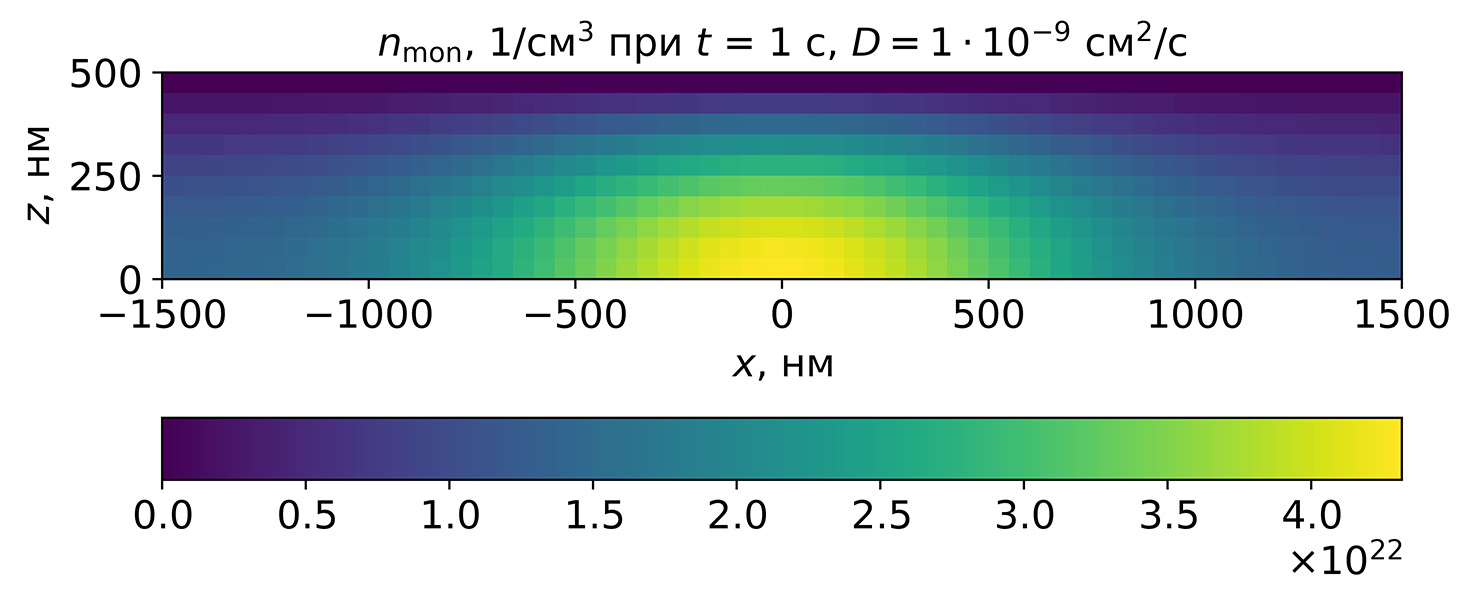
\includegraphics[width=0.8\linewidth]{diffusion/n_mon_1e-9_1s_straight_200} \\
		\vspace{-4em} \text{\hspace{-26em} б)} \vspace{2em} \\
		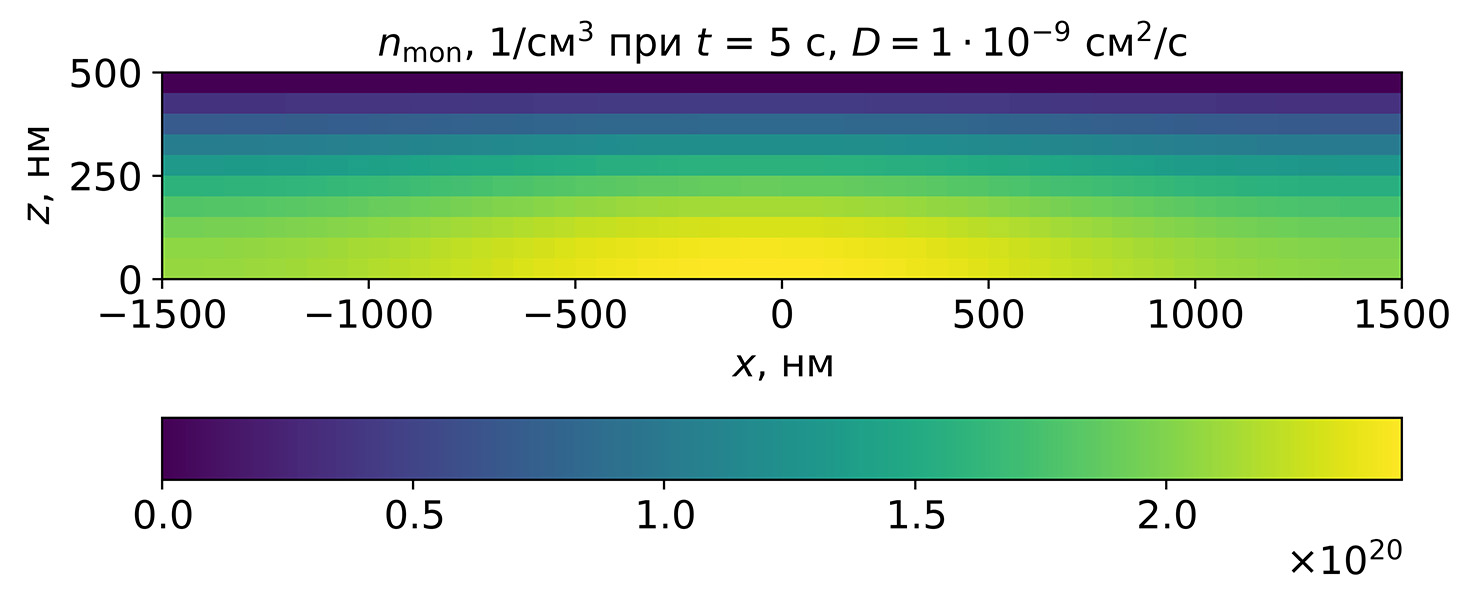
\includegraphics[width=0.8\linewidth]{diffusion/n_mon_1e-9_5s_straight_200} \\
		\vspace{-4em} \text{\hspace{-26em} в)} \vspace{2em} \\
		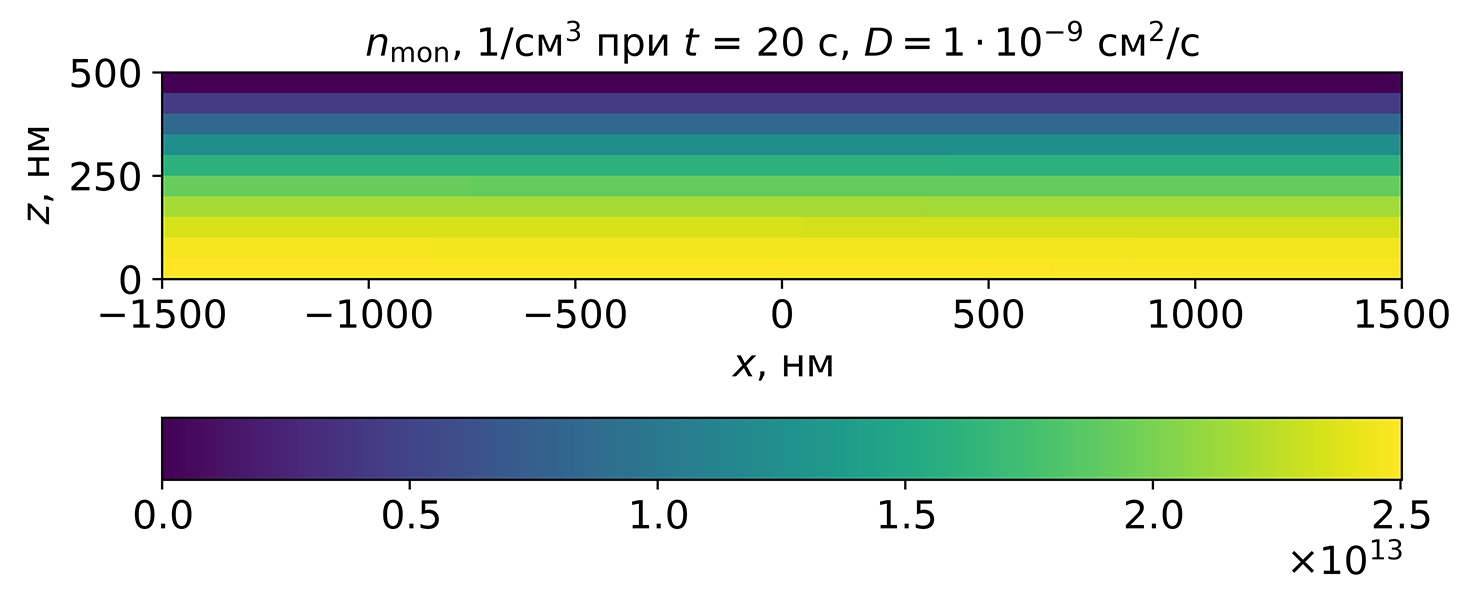
\includegraphics[width=0.8\linewidth]{diffusion/n_mon_1e-9_20s_straight_200} \\
		\vspace{-4em} \text{\hspace{-26em} г)} \vspace{2em} \\
	\end{center}
%	\vspace{-1em}
	\vspace{-1.5em}
	\caption{Моделирование диффузии мономера, образовавшегося в слое ПММА за 1~секунду в процессе СЭЛТР при температуре 135~$^\circ$C с параметрами экспонирования, описанными в разделе~\ref{sec:depolymerization}: а) начальное распределение концентрации мономера; б), в), г) распределения концентрации мономера после диффузии в течение 1, 5 и 20 с соответственно. Коэффициент диффузии составляет 1\:$\cdot$\,10$^\text{-9}$ см$\pp$/c.}
	\label{fig:diffusion_10s}
\end{figure}

\section{Модель нагрева слоя ПММА при экспонировании}

Выделение энергии в резисте при его экспонировании электронным лучом может приводить к нагреву резиста. Поскольку в методе СЭЛТР температура резиста непосредственным образом определяет интенсивность различных процессов, приводящих к формированию конечного профиля, необходимо оценить, насколько повышается температура ПММА в центре линии при экспонировании. Для этого в данной работе было использовано математическое моделирование.

Моделирование нагрева слоя ПММА проводилось на основе подхода, описанного в разделе~\ref{sec:sim_heating} для следующих условий экспонирования: ток экспонирования -- 5 нА, энергия электронного пучка -- 20 кэВ, размеры экспонируемой области -- 2.4$\times$1.9 мм$\pp$, толщина слоя ПММА -- 900 нм, число линий -- 625, расстояние между линиями -- 3 мкм, время экспонирования -- 100 с, температура образца -- 130~$^\circ$C. Для вычисления интегралов в формуле~\ref{eq:heat_final_equation} использовался метод Монте-Карло, что позволило достичь компромисса между машинным временем, необходимым для вычислений и точностью вычислений.

Результаты моделирования температуры ПММА при экспонировании показало, что увеличение температуры в центре линии составляет менее 1~$^\circ$C (рисунок~\ref{fig:heating}). Это позволило в дальнейшем считать, что при экспонировании ПММА ``в кадр'' при характерных размерах области экспонирования порядка нескольких миллиметров и токе экспонирования в диапазоне 1-10 нА повышением температуры ПММА можно пренебречь.

\begin{figure}[h!]
	\begin{center}
		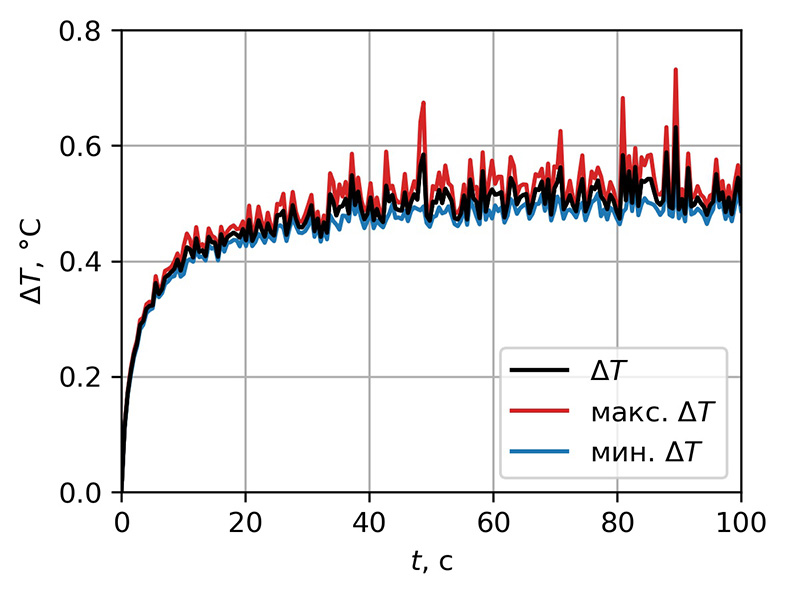
\includegraphics[width=0.6\linewidth]{heating/heating_200.jpg}
	\end{center}
	\vspace{-1em}
	\caption{Промоделированное увеличение температуры ПММА в центре линии при экспонировании ``в кадр''. Ток экспонирования -- 5 нА, энергия электронного пучка -- 20 кэВ, размеры экспонируемой области -- 2.4$\times$1.9 мм$\pp$, толщина слоя ПММА -- 900 нм, число линий -- 625, расстояние между линиями -- 3 мкм, время экспонирования -- 100 с, температура образца -- 130~$^\circ$C. Наличие минимального и максимального значений $\Delta T$ обусловлено использованием метода Монте-Карло для вычисления интегралов в формуле~\ref{eq:heat_final_equation}.}
	\label{fig:heating}
\end{figure}





\section{Модель процессов растекания в слое ПММА}

Как было показано выше, распределение среднечисловой молекулярной массы ПММА в процессе СЭЛТР является неоднородным. Следовательно, согласно формуле~\ref{eq:3p4_3p1}, распределение вязкости в слое ПММА в процессе СЭЛТР также является неоднородным. Разработанный подход моделирования распределения среднечисловой молекулярной массы ПММА вкупе с формулами~\ref{eq:WLF} и \ref{eq:3p4_3p1} позволяет промоделировать распределение вязкости ПММА в различные моменты времени в процессе СЭЛТР. Однако, существующие модели растекания не могут быть использованы в этом случае, так как в исходном виде они применимы только для однородных структур.

В данной работе для моделирования процессов растекания в слое \linebreak ПММА с неоднородным профилем вязкости был разработан численный подход на основе метода конечных элементов. В его основе лежало предположение о существовании связи между вязкостью слоя ПММА и подвижностью вершин его поверхности. Для определения характера этой связи было проведено моделирование термического растекания одной и той же структуры -- прямоугольной решетки -- аналитическим и численным методами. Период решетки и ее глубина составляли 2 мкм и 28 нм соответственно, что по порядку величин согласуется с характерными параметрами структур, получаемых литографическими методами. Вязкость материала решетки варьировалась в диапазоне 10$^\text{2}$--10$^\text{6}$ Па\:$\cdot$\,с.

Сначала растекание решетки было промоделировано аналитически, что позволило определить профиль решетки в различные моменты времени. Далее растекание решетки было промоделировано численным методом с использованием программы ``Surface Evolver'' с значением подвижности вершин поверхности решетки, равным 1. Это позволило получить значения переменной $s$, которые обеспечивали соответствие между профилями, промоделированными аналитически и численно для различных значений времени растекания при различных значениях вязкости (рисунок~\ref{fig:reflow_1} а)). При этом было установлено, что для значений вязкости материала решетки в диапазоне 10$^\text{2}$--10$^\text{6}$ Па\:$\cdot$\,с зависимости $s$ от времени растекания $t$ может быть с высокой точностью описана прямой пропорциональностью (рисунок~\ref{fig:reflow_1} б)):
\begin{equation}
	s = \alpha \cdot t.
\end{equation}
Вычисление коэффициента $\alpha$ для каждого значения вязкости позволило получить зависимость $\alpha(\eta)$, которая в логарифмических координатах оказалась практически линейной (рисунок~\ref{fig:eta_alpha}). Аппроксимация зависимости $\alpha(\eta)$ функцией вида
\begin{equation}
	\alpha = C / \eta^\beta
\end{equation}
изображена на рисунке~\ref{fig:eta_alpha}, параметры $C$ и $\beta$ составили 26.14 и 0.989, соответственно (для значения вязкости в единицах СИ).

\begin{figure}[t]
	\begin{minipage}{0.5\textwidth}
		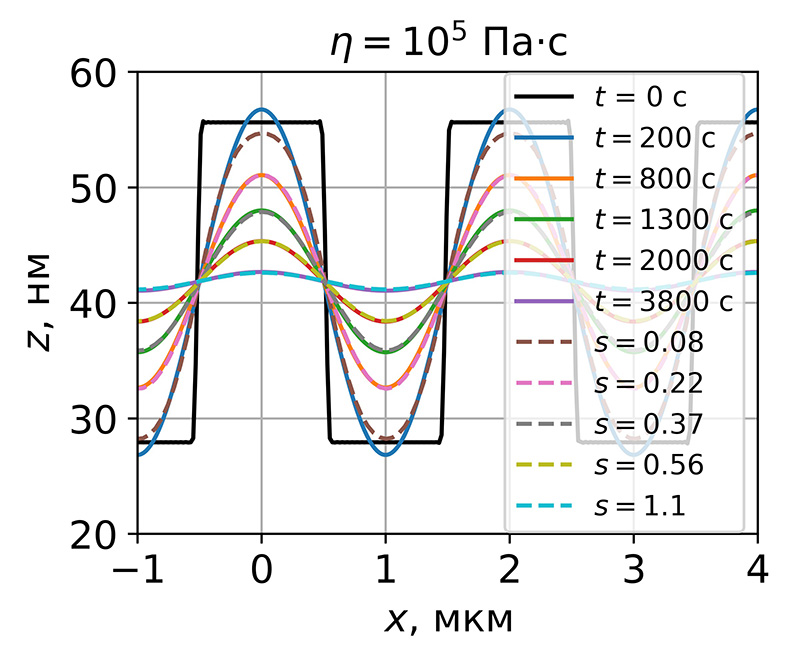
\includegraphics[width=0.91\linewidth]{reflow/grating_eta_100000_14_CORR_200} \\
		\vspace{-28.5ex} \\ \text{\hspace{0em} a}) \\ \vspace{28.5ex}
	\end{minipage}
	\begin{minipage}{0.5\textwidth}
		\hspace{-1em} 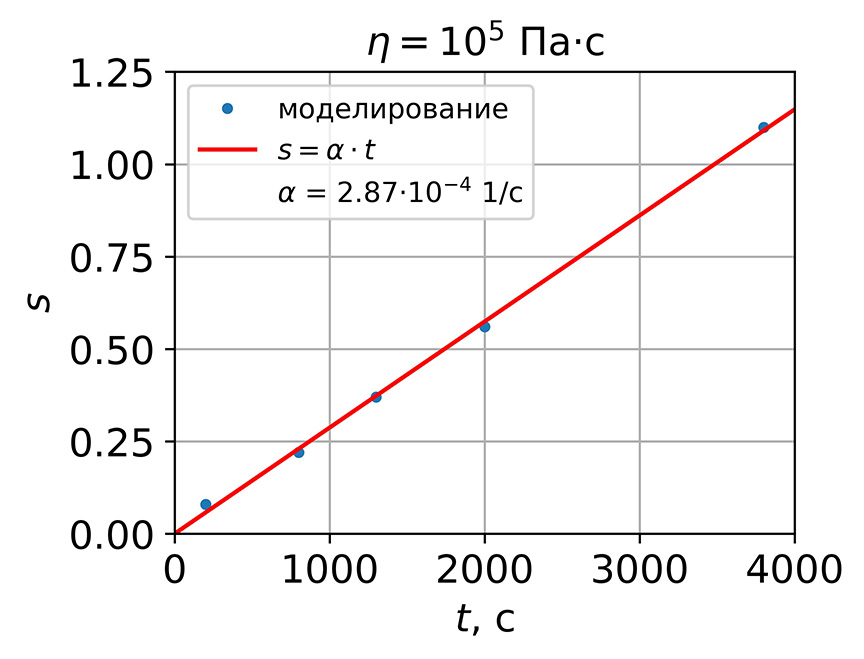
\includegraphics[width=\linewidth]{reflow/alpha_100000_14_up_200} \\
		\vspace{-28.5ex} \\ \text{\hspace{-0.8em} б}) \\ \vspace{28.5ex}
	\end{minipage}
	\vspace{-3.5em}
	\caption{Моделирование растекания прямоугольной решетки с периодом 2 мкм и глубиной 28 нм аналитическим и численным методами. Вязкость материала решетки составляет 10$^\text{5}$ Па\:$\cdot$\,с.}
	\label{fig:reflow_1}
\end{figure}

\begin{figure}[h]
	\begin{center}
		\includegraphics[width=0.6\textwidth]{reflow/С_gamma_12_SI_200}
	\end{center}
	\vspace{-1.2em}
	\caption{Рассчитанная зависимость коэффициента $\alpha$ от вязкости материала решетки.}
	\label{fig:eta_alpha}
\end{figure}

Данная зависимость была использована для определения значений подвижности вершин поверхности решетки для различных значений вязкости материала решетки. При численном моделировании растекания образца программа ``Surface Evolver'' позволяет отслеживать значение параметра $s$, и логично потребовать, чтобы это значение в точности соответствовало времени растекания. Учитывая уравнения~\ref{eq:SE_v}, \ref{eq:SE_v}, в этом случае подвижность вершин поверхности решетки ($\mu$) может быть выражена следующим образом:
\begin{equation}
	\mu = t / s \equiv \alpha.
\end{equation}
Следовательно, полученная выше зависимость $\alpha(\eta)$ является искомой зависимостью подвижности вершин поверхности резиста от его вязкости, при которой значение переменной $s$ будет в точности соответствовать времени растекания:
\begin{equation}
	\mu(\eta) \approx \frac{26.14}{\eta}.
\end{equation}
Найденная зависимость позволяет промоделировать растекание сплошной структуры в резисте с неоднородным (в плоскости $XY$) профилем вязкости: сначала на основе распределения вязкости рассчитываются подвижности вершин поверхности структуры, затем в программе ``Surface Evolver'' задается поверхность с нужными значениями подвижности вершин и далее производится моделирование эволюции поверхности в заданном промежутке значений переменной $s$.

Однако, слой ПММА в процессе СЭЛТР не только имеет неоднородный профиль вязкости, но является неоднородным в целом.
Как уже было отмечено, в процессе термической деполимеризации в слое ПММА образуется большое количество свободного мономера, который быстро покидает область травления.
Это приводит к появлению микрополостей, объем которых может быть вычислен по формуле
\begin{equation}
	V_\mathrm{cav} = N_\mathrm{sci} \cdot 1/\gamma \cdot V_\mathrm{mon},
\end{equation}
где $N_\text{sci}$ -- число разрывов молекул ПММА в некоторой области, $1/\gamma$ -- средняя длина кинетической цепи при деполимеризации, $V_\mathrm{mon}$ -- средний объем одного мономера ($\approx$ 0.14 нм$\ppp$).
Процессы растекания в методе СЭЛТР протекают за счет действия сил поверхностного натяжения на границах микрополостей в слое ПММА, и для возможности применения разработанного подхода для моделирования такого растекания использовалось следующее приближение.
Слой ПММА разделялся в плоскости $XY$ на участки размерами 100$\times$100 нм$\pp$, и для каждого участка на основе промоделированного распределения разрывов молекул ПММА и средней длины кинетической цепи при деполимеризации рассчитывались положения и объемы микрополостей.
Далее точки поверхности слоя ПММА, соответствующие середине каждого участка по оси $X$, сдвигались вниз таким образом, чтобы объем призмы, образующейся под поверхностью слоя ПММА, был равен суммарному объему микрополостей на этом участке (рисунок~\ref{fig:reflow_surface}).
Полученная пилообразная структура задавалась в программе ``Surface Evolver'' со значениями подвижности вершин, рассчитанными из распределения вязкости ПММА.
После этого растекание данной структуры моделировалось в течение нужного промежутка времени.

\begin{figure}[h]
	\begin{minipage}{0.48\textwidth}
		\includegraphics[width=0.9\linewidth]{reflow/reflow_model_a_CIRCLES_4} \\
		\vspace{-28.5ex} \\ \text{\hspace{0em} a}) \\ \vspace{28.5ex}
	\end{minipage}
	\begin{minipage}{0.48\textwidth}
		\includegraphics[width=0.9\linewidth]{reflow/reflow_model_b} \\
		\vspace{-28.5ex} \\ \text{\hspace{-0.1em} б}) \\ \vspace{28.5ex}
	\end{minipage}
	\vspace{-3.5em}
	\caption{Иллюстрация подхода к моделированию растекания слоя ПММА со внутренними микрополостями.}
	\label{fig:reflow_surface}
\end{figure}

\section{Модель сухого электронно-лучевого травления резиста.}

Объединение моделей рассеяния электронного пучка, электронно-стимулированных разрывов молекул ПММА, электронно-стимулированной деполимеризации ПММА, диффузии мономера и растекания ПММА позволило создать модель процесса СЭЛТР. На ее основе был разработан алгоритм моделирования профиля линии, получаемой методом СЭЛТР при произвольных параметрах процесса. В данном алгоритме все время экспонирования разбивалось на промежутки величиной 1~с, и на каждом промежутке последовательно выполнялись следующие действия:

\begin{enumerate}
	\item Моделирование рассеяния электронного пучка в системе ПММА/Si;
	\item Моделирование электронно-стимулированных разрывов молекул \linebreak ПММА;
	\item Моделирование термической деполимеризации ПММА;
	\item Определение подвижностей вершин поверхности слоя ПММА;
	\item Вычисление положений и объемов микрополостей в слое ПММА;
	\item Преобразование слоя ПММА со внутренними микрополостями в сплошную пилообразную структуру;
	\item Моделирование растекания пилообразной структуры;
	\item Определение нового положения поверхности слоя ПММА.
\end{enumerate}

По истечении времени экспонирования также моделировалось растекание слоя ПММА при его охлаждении до температуры, при которой процессы растекания переставали протекать заметным образом (было установлено, что эта температура составляет около 80 $^\circ$C).

Демонстрация процесса моделирования профиля линии, получаемой методом СЭЛТР, приведена на рисунке~\ref{fig:DEBER_example}. Моделирование проводилось для следующих условий условий процесса СЭЛТР: начальная толщина слоя ПММА равна 500~нм, энергия электронного пучка $E$ = 20 кэВ, температура образца $T$~=~150~$^{\circ}$C/c, время экспонирования $t_\mathrm{exp}$ = 100 с, плотность тока экспонирования на единицу длины $j_\mathrm{l}$ = 10 пА/см, скорость охлаждения образца после экспонирования составляла 1~$^{\circ}$C/с.

\begin{figure}[t!]
	\begin{minipage}{0.48\textwidth}
		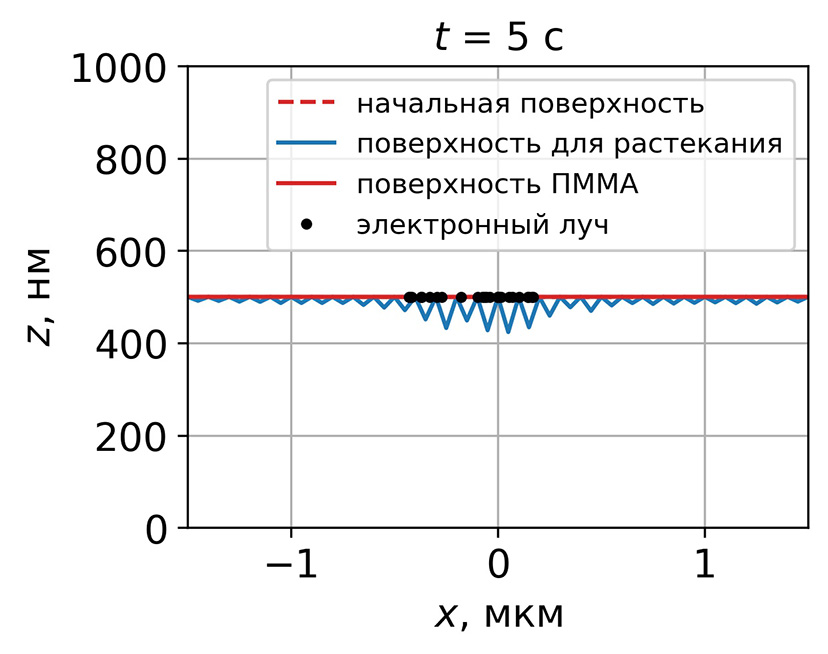
\includegraphics[width=\linewidth]{DEBER_example/example_5_200} \\
		\vspace{-13em} \\ \text{\hspace{0em} a}) \\ \vspace{13em}
	\end{minipage}
	\begin{minipage}{0.48\textwidth}
		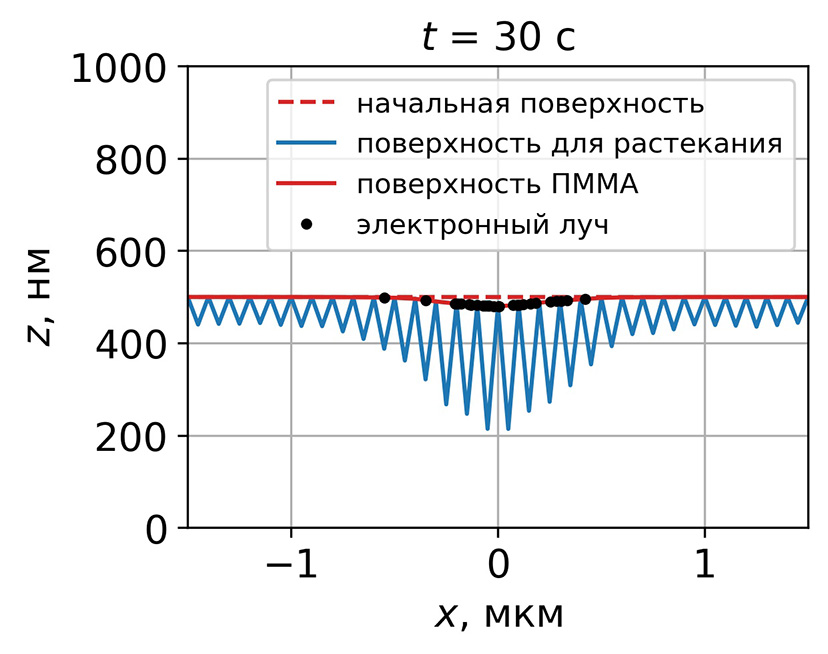
\includegraphics[width=\linewidth]{DEBER_example/example_30_200} \\
		\vspace{-13em} \\ \text{\hspace{-0.1em} б}) \\ \vspace{13em}
	\end{minipage}
	
	\vspace{-3em}
	
	\begin{minipage}{0.48\textwidth}
		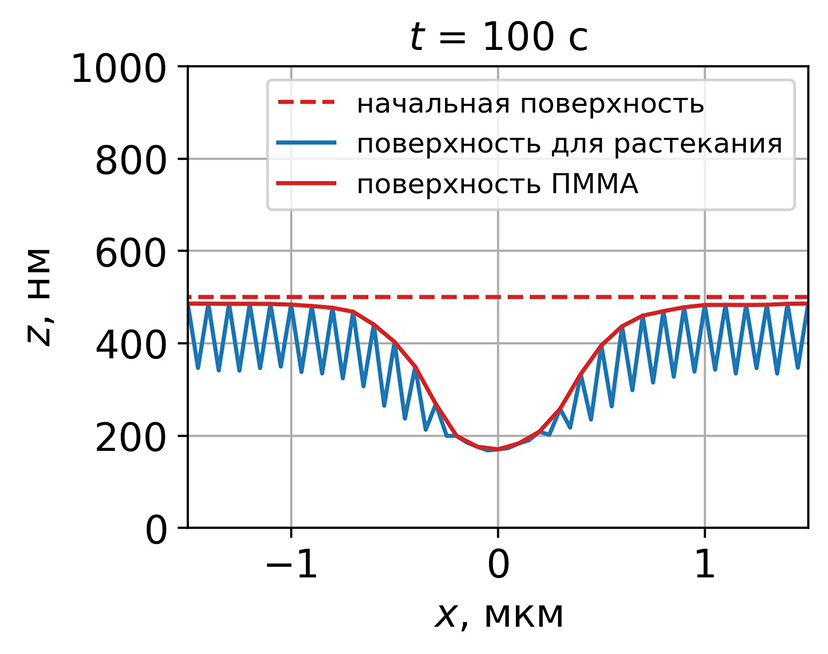
\includegraphics[width=\linewidth]{DEBER_example/example_100_200} \\
		\vspace{-13em} \\ \text{\hspace{0em} в}) \\ \vspace{13em}
	\end{minipage}
	\begin{minipage}{0.48\textwidth}
		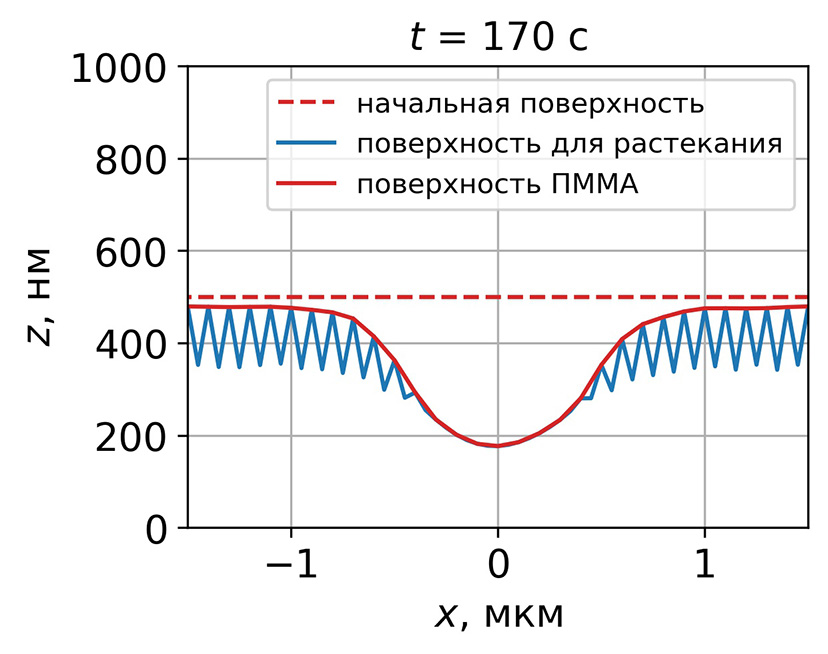
\includegraphics[width=\linewidth]{DEBER_example/example_170_200} \\
		\vspace{-13em} \\ \text{\hspace{-0.1em} г}) \\ \vspace{13em}
	\end{minipage}
	\vspace{-3em}
	\caption{Моделирование профиля линии, получаемой методом СЭЛТР, в различные моменты времени в течение процесса экспонирования и охлаждения образца. Условия экспонирования: $E$ = 20 кэВ, $T$ = 150 $^{\circ}$C/c, $t_\mathrm{exp}$ = 100 с, плотность тока экспонирования на единицу длины $j_\mathrm{l}$ = 10 пА/см, скорость охлаждения образца -- 1~$^{\circ}$C/с. Красная пунктирная линия обозначает начальное положение поверхности слоя ПММА, черные точки -- координаты точек входа электронного пучка в слой резиста.}
	\label{fig:DEBER_example}
\end{figure}

На основе моделирования процесса СЭЛТР можно сделать следующие общие заключения о процессе формирования линии в данном процессе. В начальные моменты времени экспонирование резиста приводит к его деполимеризации и появлению в нем микрополостей, однако, процессы растекания еще не могут протекать заметным образом за счет большой вязкости резиста (рисунок~\ref{fig:DEBER_example},~a)). При дальнейшем экспонировании молекулярная масса и, соответственно, вязкость резиста снижаются до значений, при которых становится возможным заметное растекание резиста и заполнение микрополостей (рисунок~\ref{fig:DEBER_example},~б)). С этого момента времени процессы деполимеризации резиста, уменьшения его вязкости, образования новых микрополостей и заполнения старых протекают одновременно до окончания экспонирования. При окончании экспонирования прекращается образование новых микрополостей и уменьшение вязкости резиста, и дальнейшее охлаждение образца сопровождается только заполнением существующих микрополостей (рисунок~\ref{fig:DEBER_example}, в)). С уменьшением температуры образца вязкость резиста увеличивается, и процессы растекания затухают (рисунок~\ref{fig:DEBER_example}, г)).


\section{Экспериментальные методы}

Для оценки достоверности разработанной модели СЭЛТР должна быть проведена ее верификация на основе профилей, полученных экспериментально. В этом разделе описаны подходы, применявшиеся при формировании структур методом СЭЛТР и получении профилей этих структур.

\subsection*{Растровая электронная микроскопия}

В растровой электронной микроскопии (РЭМ) изображение объекта формируется последовательно по точкам, каждая из которых получается за счет облучения поверхности объекта сфокусированным электронным пучком. При взаимодействии первичных электронов с веществом возникают вторичные сигналы различной физической природы -- отраженные и вторичные электроны, Оже-электроны, рентгеновское излучение, свет, поглощенный ток и пр. (рисунок~\ref{fig:REM_1}), которые регистрируются соответствующими датчиками. Регистрируемый сигнал используется в дальнейшем для формирования изображения сканируемой поверхности на экране монитора. Величины вторичных сигналов зависят от физических свойств поверхности исследуемого образца и могут изменяться от точки к точке. В результате на экране монитора образуется изображение поверхности образца, отображающее топографию соответствующего физического свойства. За счет этого можно исследовать топологию поверхности -- в обратно отраженных или вторичных электронах; распределение элементного состава по поверхности образца -- в характеристическом рентгеновском излучении; распределение донорных или акцепторных центров -- по величине поглощенного тока; топографию магнитной доменной структуры -- во вторичных электронах и пр.

\begin{figure}
	\centering
	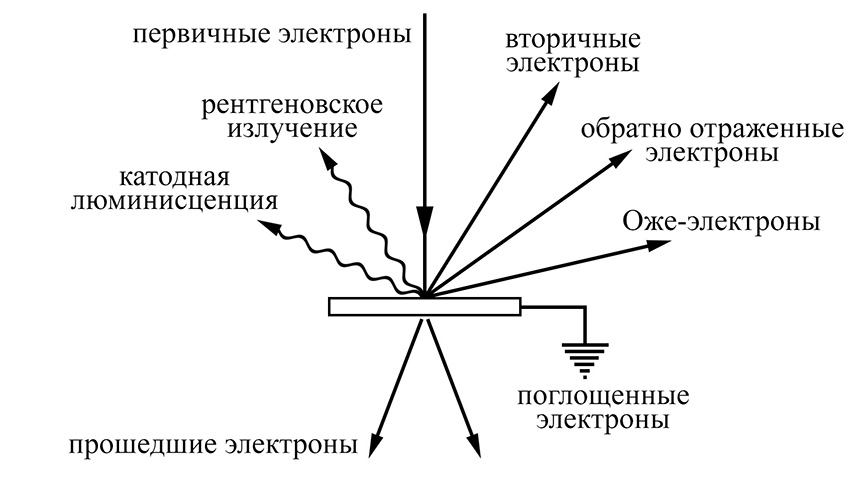
\includegraphics[width=0.95\textwidth]{experiment/REM_1_small}
	\caption{Схема образования вторичных сигналов при взаимодействии электронного пучка с веществом мишени.}
	\label{fig:REM_1}
\end{figure}

Растровый электронный микроскоп является вакуумным прибором, так как при нормальном атмосферном давлении электронный пучок сильно рассеивается и поглощается, что делает невозможным его фокусировку. Давление в рабочей камере микроскопа должно составлять порядка 10$^\text{-5}$ торр или ниже. Схема основных элементов растрового электронного микроскопа приведена на рисунке~\ref{fig:REM_2}. Электронный пучок от источника электронов фокусируется специальной конденсорной системой и проходит через систему управляющих электродов или электромагнитов, которые перемещают пучок по поверхности образца по траектории, образующей растр.

\begin{figure}[t]
	\centering
	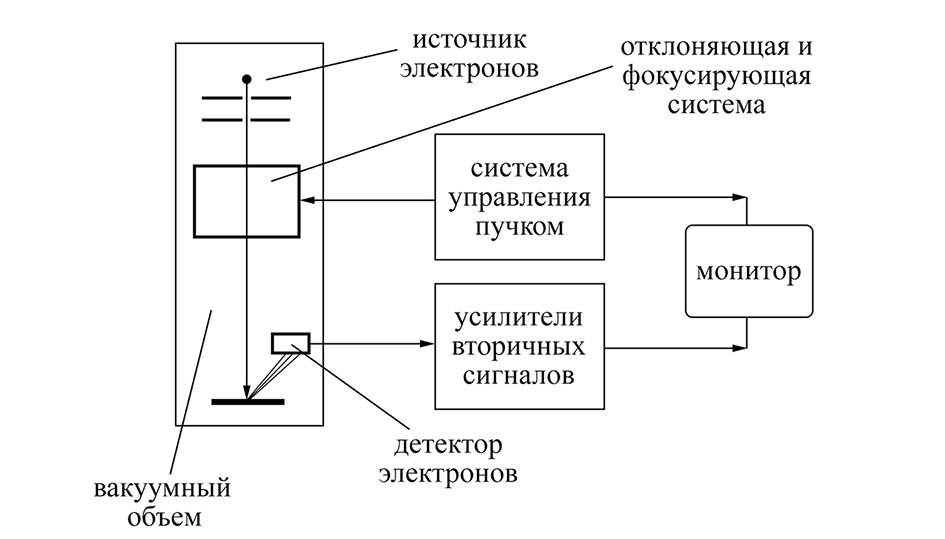
\includegraphics[width=0.95\textwidth]{experiment/REM_2_200}
	\caption{Упрощенная схема, иллюстрирующая работу РЭМ.}
	\label{fig:REM_2}
\end{figure}

Разрешение РЭМ определяется размером области в образце, возбуждаемой электронным пучком, а интенсивность вторичных сигналов --  величиной тока пучка. Таким образом, электронно-оптическая система, формирующая пучок, должна обеспечивать получение максимально возможного тока при минимально возможных поперечных размерах пучка. Электронно-оптическая система включает в себя источник электронов (вольфрамовый катод, катод из гексаборида лантана (LaB$_\text{6}$) или автоэмиссионный катод), модулятор (цилиндра Венельта) и анод (рисунок~\ref{fig:REM_3}). Модулятор обычно имеет отрицательный потенциал в несколько сотен вольт относительно катода, что позволяет сформировать электронный пучок с диаметром $d_0$ и расходимостью $\alpha_0$. Характерные значения $d_0$ и $\alpha_0$ для электронно-оптических систем, используемых в рентгеновских микроанализаторах и растровых электронных микроскопах, составляют 25--100 мкм и 3--10\:$\cdot$\,10$^\text{-3}$ рад соответственно.

\begin{figure}
	\centering
	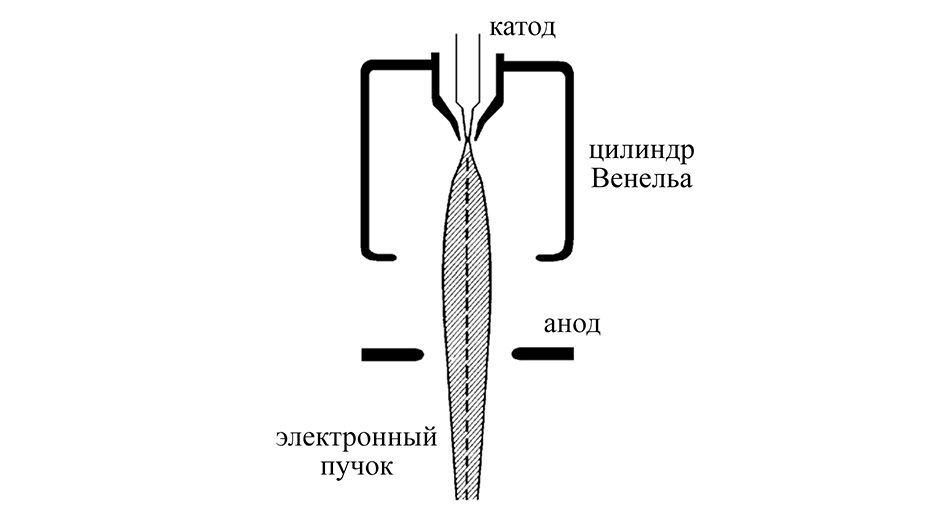
\includegraphics[width=0.95\textwidth]{experiment/REM_3_200}
	\caption{Схема устройства электронно-оптической системы растрового электронного микроскопа.}
	\label{fig:REM_3}
\end{figure}

\paragraph{Сцинтилляционный детектор} \mbox{} \\
\indent В настоящее время наиболее широкое распространение в РЭМ для регистрации вторичных электронов получили сцинтилляционные детекторы. Вторичные электроны попадают на сцинтиллятор, преобразующий энергию электрона в световой импульс, который улавливается фотокатодом, преобразуется в фототок и затем усиливается фотоэлектронным умножителем. Между сцинтиллятором и фотоэлектронным умножителем помещается световод, позволяющий вывести фотоумножитель, крайне чувствительный к внешним электрическим и магнитным полям, за пределы вакуумной камеры РЭМ. Так как большинство используемых сцинтилляторов генерируют свет под действием электронов с энергией более 10 кэВ, на внешнюю поверхность сцинтиллятора наносится тонкий полупрозрачный металлический слой, и на него подается положительное напряжение (порядка 10 кВ) для сбора и ускорения низкоэнергетической части спектра вторичных электронов. Для того, чтобы исключить влияние созданного электрического поля на первичные электроны, сцинтиллятор помещается внутрь цилиндра Фарадея. 

\paragraph{Полупроводниковый детектор} \mbox{} \\
\indent Вторичные электроны, попавшие в материал полупроводника вблизи \textit{p-n}-перехода, обеспечивают образование в нем электронно-дырочных пар, что приводит к появлению тока через \textit{p-n}-переход. Этот ток пропорционален количеству электронов, поглощенных полупроводником. Для получения достаточной величины сигнала ток в дальнейшем усиливается специальными малошумящими усилителями. Электроны должны иметь энергию, достаточную для образования электронно-дырочных пар, поэтому полупроводниковый детектор (ППД) обычно используется для регистрации высокоэнергетической части вторичных электронов.

\paragraph{Детектор излучения катодолюминесценции} \mbox{} \\
\indent Количество света, испускаемого мишенью под воздействием электронного пучка, обычно мало, поэтому для увеличения эффективности регистрации испускаемого света используют специальные эллиптические зеркала. В один из фокусов зеркала помещают мишень, а в другой -- световод-приемник, уводящий свет за пределы вакуумной камеры микроскопа. Далее свет регистрируется фотоэлектронным умножителем, либо спектрометром, позволяющим исследовать распределение испущенного образцом света по длинам волн.

\paragraph{Детекторы рентгеновского излучения} \mbox{} \\
\indent Для регистрации рентгеновского излучения обычно используются два типа систем. Во-первых, применяются кристалл-дифракционные спектрометры с изогнутыми для увеличения светосилы кристаллами-анализаторами. Приемником рентгеновского излучения обычно служит сцинтилляционный детектор. В качестве кристалла-сцинтиллятора обычно используются монокристаллы NaI(Tl). Во-вторых, также применяются энергодисперсионные системы, например, кремний-литиевые детекторы. Энергодисперсионные детекторы имеют существенно более низкое энергетическое разрешение (100--150 эВ) по сравнению с кристалл-дифракционными спектрометрами (менее 10 эВ), однако они получили широкое распространение благодаря возможности регистрации всего спектра вторичных электронов без каких-либо перемещений образца и детектора, а также возможности быстрой обработки спектра на ЭВМ.


\subsection*{Атомно-силовая микроскопия}

В основе принципа работы атомно-силового микроскопа (АСМ) лежит силовое взаимодействие между сторонним телом и поверхностью вещества, для регистрации которого используются специальные датчики, представляющие собой упругую консоль (кантилевер) с острым зондом на конце (рисунок~\ref{fig:AFM_1_2} а)). Сила, действующая на зонд со стороны поверхности, приводит к изгибу кантилевера, и за счет регистрации величины изгиба в разных точках сканируемой поверхности можно определить профиль поверхности.

Качественно работу АСМ можно пояснить на примере сил Ван-дер-Ваальса. Энергия ван-дер-ваальсова взаимодействия двух атомов, находящихся на расстоянии $r$ друг от друга, может быть аппроксимирована потенциалом Леннарда-Джонса (рисунок ~\ref{fig:AFM_1_2} б)):
\begin{equation}
	U_\mathrm{LJ}(r) = U_0\left\{-2\left(\frac{r_0}{r}\right)^6+\left(\frac{r_0}{r}\right)^{12}\right\}.
\end{equation}
Первое слагаемое в скобках описывает дальнодействующее притяжение, обусловленное, диполь-дипольным взаимодействием атомов, второе -- отталкивание атомов на малых расстояниях. Параметр $r_0$ -- равновесное расстояние между атомами, $U_0$ -- значение энергии в положении равновесия. 

Полная энергия системы зонд-образец задается формулой
\begin{equation}
	W_\mathrm{PS}=\iint_{\mathrm{V}_\mathrm{P} \mathrm{V}_\mathrm{S}} U_\mathrm{LJ}\left(r-r^{\prime}\right) n_\mathrm{P}\left(r^{\prime}\right) n_\mathrm{S}(r) d V d V^{\prime}
\end{equation}
где $n_\mathrm{P}(r)$ и $n_\mathrm{S}(r^\prime)$ -- плотности атомов в материале зонда и образца, соответственно. Соответственно, сила, действующая на зонд со стороны поверхности, может быть вычислена следующим образом:
\begin{equation}
	\vec{F}_\mathrm{PS} = -\operatorname{grad}\left(W_\mathrm{PS}\right).
\end{equation}
Такое взаимодействие зонда с образцом имеет сложный характер, однако основные черты взаимодействия, характерного для двух атомов, сохраняются -- зонд АСМ испытывает притяжение со стороны образца на больших расстояниях от его поверхности и отталкивание -- на малых.

Получение изображения рельефа поверхности с помощью АСМ связано с регистрацией малых изгибов упругой консоли зондового датчика, для чего широко используются оптические методы (рисунок~\ref{fig:AFM_2}). Оптическая система АСМ юстируется таким образом, чтобы излучение полупроводникового лазера фокусировалось на консоли зондового датчика, а отраженный пучок попадал в центр фоточувствительной области фотоприемника. В качестве позиционно-чувствительных фотоприемников применяются четырехсекционные полупроводниковые фотодиоды.

\begin{figure}[t]
	\centering
	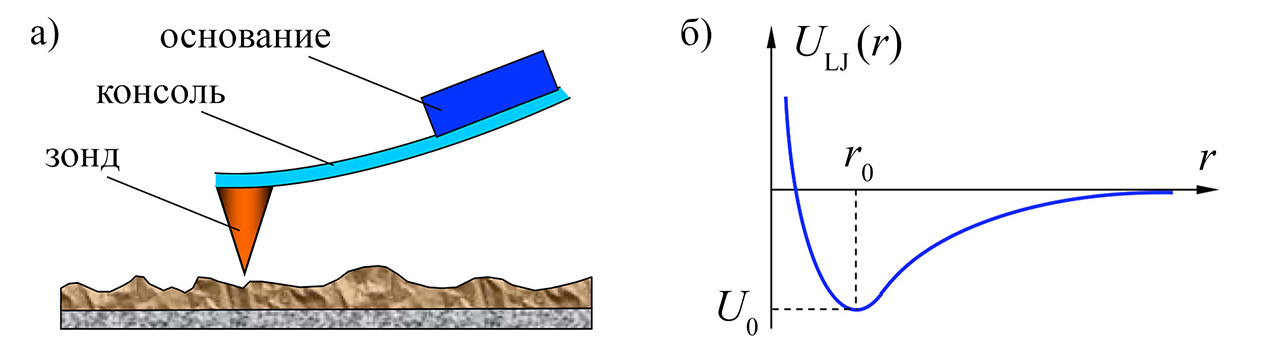
\includegraphics[width=0.9\textwidth]{experiment/AFM_1_2_200}
	\vspace{0.5em}
	\caption{а) Схематическое изображение зондового датчика АСМ, б) качественный вид потенциала Леннарда-Джонса.}
	\label{fig:AFM_1_2}
\end{figure}

Основные регистрируемые оптической системой параметры -- это деформации изгиба консоли под действием $Z$-компонент сил притяжения или отталкивания ($F_\mathrm{Z}$) и деформации кручения консоли под действием латеральных компонент сил ($F_\mathrm{L}$) взаимодействия зонда с поверхностью. Если обозначить исходные значения фототока в секциях фотодиода через $I_{01}$, $I_{02}$, $I_{03}$, $I_{04}$, а через $I_{1}$, $I_{2}$, $I_{3}$, $I_{4}$ -- значения токов после изменения положения консоли, то разностные токи с различных секций фотодиода $\Delta I_i = I_i - I_{0i}$ будут однозначно характеризовать величину и направление изгиба консоли зондового датчика АСМ. Действительно, комбинация разностных токов вида
\begin{equation}
	\Delta I_\mathrm{Z} = \left(\Delta I_1+\Delta I_2\right)-\left(\Delta I_3+\Delta I_4\right)
\end{equation}
пропорциональна изгибу консоли под действием силы, действующей по нормали к поверхности образца, а комбинация вида
\begin{equation}
	\Delta I_\mathrm{L} = \left(\Delta I_1+\Delta I_4\right)-\left(\Delta I_2+\Delta I_3\right)
\end{equation}
характеризует изгиб консоли под действием латеральных сил.

\begin{figure}[t]
	\centering
	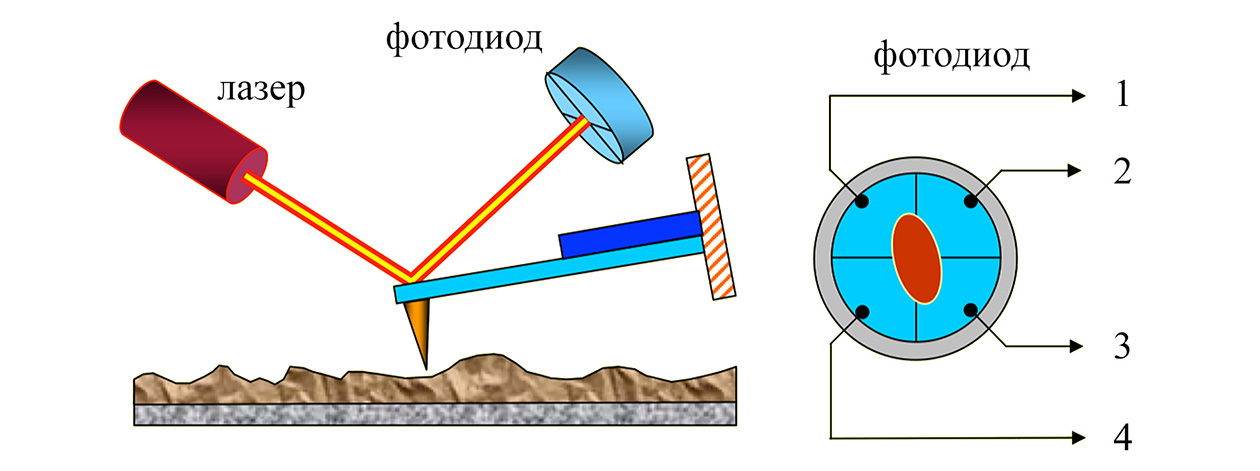
\includegraphics[width=0.9\textwidth]{experiment/AFM_3_200}
	\vspace{0.2em}
	\caption{Схема оптической регистрации изгиба консоли зондового датчика АСМ.}
	\label{fig:AFM_2}
\end{figure}

Величина $\Delta I_\mathrm{Z}$ используется в качестве входного параметра в петле обратной связи атомно-силового микроскопа. Система обратной связи обеспечивает постоянное значение $\Delta I_\mathrm{Z}$ с помощью пьезоэлектрического исполнительного элемента, который поддерживает изгиб консоли $\Delta Z$ равным величине $\Delta Z_0$, задаваемой оператором.

При сканировании образца в режиме $\Delta Z = const$ зонд перемещается вдоль поверхности, при этом напряжение на $Z$-электроде сканера записывается в память компьютера в качестве рельефа поверхности $Z = f(X, Y)$. Пространственное разрешение АСМ определяется радиусом закругления зонда и чувствительностью системы, регистрирующей отклонения консоли. В настоящее время реализованы конструкции АСМ, позволяющие исследовать поверхность образцов с атомарным разрешением.


